% !TeX program = xelatex
\documentclass[fleqn,10pt]{wlpeerj}

\usepackage{fontspec}
\usepackage{booktabs}
\usepackage{longtable}
\usepackage{array}
\usepackage{calc}
\usepackage{amsmath}
\usepackage{amssymb}
\usepackage{enumitem}
\usepackage{graphicx}
\usepackage[hidelinks]{hyperref}
\providecommand{\tightlist}{\setlength{\itemsep}{0pt}\setlength{\parskip}{0pt}}

\title{A Quantified Safety--Accuracy Trade-off: Margin-Ranking and Severity-Weighted LoRA Fine-Tuning for Look-Alike/Sound-Alike Drug Name Errors in Handwritten Prescription OCR}

\author[1]{Bang Dang}
\affil[1]{Independent Researcher}
\corrauthor[1]{Bang Dang}{bangdang007112@gmail.com}

\keywords{optical character recognition, handwritten prescription recognition, LoRA (Low-Rank Adaptation) fine-tuning, look-alike/sound-alike (LASA) drug names, medication safety, margin-ranking loss, severity-weighted loss, safety-accuracy trade-off}

\begin{abstract}
Low-Rank Adaptation (LoRA) fine-tuning of transformer-based optical character recognition (OCR) models improves overall handwriting-recognition accuracy, but a related, independent study found that fine-tuning a sequence-to-sequence OCR model on handwritten medical text can simultaneously increase a specific, clinically dangerous error type: misreading one real drug name as a different real drug name, a look-alike/sound-alike (LASA) confusion that a pharmacist can mistake for a valid prescription. We independently reproduced this trade-off on two new public datasets (Kaggle-BD, 78 drug classes; RxHandBD, a larger and more LASA-rich vocabulary) with zero-shot and LoRA-fine-tuned TrOCR, and we derived confusable drug-name candidates directly from each dataset's own vocabulary with a lexicon-free edit-distance/phonetic similarity score (BI-SIM), avoiding any curated clinical LASA list. We used these candidates to train LoRA with a combined margin-ranking and severity-weighted cross-entropy loss, evaluated in a two-phase design: an exploratory, single-run hyperparameter sweep that selected one configuration, followed by a confirmatory replication of that configuration across five independently seeded training runs, each paired against a matched cross-entropy-only baseline. On RxHandBD, the confirmatory replication (pooled paired McNemar tests, n = 5,575) shows that the selected loss reduces the LASA (confusable\_wrong\_drug) error rate by 0.90 percentage points (95\% CI [-1.34, -0.46]; \textasciitilde12.6\% relative), but at a statistically robust cost: overall correct-prediction rate falls by 2.01 points (95\% CI [-2.80, -1.22]) and hallucination-type errors rise by 2.15 points (95\% CI [1.39, 2.92]), with all three metrics moving in the same direction in all 5 of 5 seeds. A destination-of-errors analysis shows most resolved LASA errors become clearly wrong rather than correct, and few correct predictions turn newly dangerous. This intervention did not replicate on the smaller, closed-vocabulary Kaggle-BD dataset. We therefore present this loss combination as a quantified, disclosed operating point on a safety--accuracy trade-off curve for large, LASA-rich prescription vocabularies, not as a cost-free improvement.
\end{abstract}

\begin{document}

\flushbottom
\maketitle
\thispagestyle{empty}

\section*{Introduction}\label{sec:introduction}

Handwritten medical prescriptions remain common in many health systems, and automatic transcription of them --- optical character recognition (OCR) applied to clinical handwriting --- is a natural target for record digitization and for downstream safety checks before a prescription reaches a pharmacy. Not every OCR error carries the same clinical weight, however. An output that is obviously garbled is easy for a pharmacist to flag and set aside. An error in which the model outputs a different, but equally real, drug name is a different kind of failure: it produces a fluent, valid-looking prescription for the wrong medication, and is correspondingly harder to catch on routine review. This class of error --- ``look-alike, sound-alike'' (LASA), or confusable-drug-name, confusion --- is a well-recognized, actively studied category of medication error in its own right, arising from orthographic and phonetic similarity between otherwise unrelated drug names and compounded by similar packaging, dosage form, or route of administration \citep{bryan2021problem}; it is treated in the pharmacy-informatics and computational-linguistics literature as a distinct problem worth its own detection methodology, independent of raw transcription accuracy \citep{kondrak2004identification,kondrak2006automatic}.

A prior, separate project by the author examined this problem for OCR directly: fine-tuning TrOCR with Low-Rank Adaptation (LoRA) on handwritten medical text reduced wildly-wrong, non-word (``hallucination'') errors overall, but specifically increased the rate at which the model misread one real drug name as a \emph{different} real drug name --- the confusable-drug-name category described above \citep{dang2026zeroshot}. That finding rests on a different dataset, label set, and codebase than the present study, and we cite it here strictly as motivating context for the research question below, not as evidence this paper itself produced.

The present study asks two questions that finding raises but does not answer. First, does the same pattern --- overall transcription accuracy improving while the single most dangerous error type gets worse --- reproduce independently, on new public data, with a new, unrelated implementation? Second, if the loss function used during fine-tuning is partly responsible for this pattern, can the loss itself be modified to discourage the dangerous error category directly, rather than relying on a post-hoc filter to catch it afterward?

We address the first question with a zero-shot-versus-fine-tuned reproduction on two public datasets. On Kaggle-BD (a 78-class closed vocabulary, n = 780 test images), zero-shot TrOCR reaches 22.95\% correct (179/780) with a confusable-wrong-drug rate of 0.38\% (3/780); a single-run LoRA cross-entropy (CE)-only fine-tune raises correct predictions to 87.95\% (686/780) while the confusable-wrong-drug rate stays at 0.64\% (5/780) --- a shift from 3 to 5 affected images, too small a sample on its own to read as a meaningful change. On RxHandBD, a larger and more LASA-rich vocabulary (approximately 1,430 normalized label instances, n = 1,115 test images), the same comparison tells a different story. Zero-shot TrOCR reaches only 19.55\% correct (218/1,115); LoRA CE-only fine-tuning raises correct predictions to 46.64\% (520/1,115) and cuts far-off hallucination from 60.90\% to 22.15\% --- but the confusable-wrong-drug rate rises from 1.79\% (20/1,115) to 7.26\% (81/1,115), roughly a four-fold relative increase. A second, independent CE-only fine-tuning run gave a consistent result (confusable-wrong-drug 7.44\%, 83/1,115; correct 46.5\%, 519/1,115), which we treat as ordinary run-to-run variation rather than a discrepancy --- and it is exactly this kind of variation that later motivated the fully-seeded confirmatory design described below. Taken together, these results reproduce, on new public data and a codebase unrelated to the prior project's, the same central paradox: fine-tuning improves overall accuracy sharply while making the single most dangerous error type worse --- and it does so specifically in the setting with a larger, more confusable-rich drug vocabulary, consistent with the effect depending on vocabulary size and LASA density rather than being a fixed property of LoRA fine-tuning in general.

Having reproduced the phenomenon, we test whether it can be addressed inside the fine-tuning loss itself rather than through post-hoc filtering. We add two terms on top of standard cross-entropy: a severity-weighted CE term, adapted from a risk-calibrated loss originally proposed for single-label medical-image classification, and a margin-ranking term that trains the model to score the true label ahead of an algorithmically-derived confusable neighbor by a fixed margin. Critically, we do not treat a favorable result from a single exploratory hyperparameter-sweep run as sufficient evidence that this intervention works. An earlier internal draft of this manuscript did exactly that --- reporting, from the one exploratory run that selected it, that the chosen configuration reduced the confusable-wrong-drug rate ``without a significant cost'' to accuracy or hallucination. A subsequent five-seed, fully-seeded confirmatory replication overturned that framing: the apparent free improvement was a favorable statistical outlier, not a property of the configuration. We therefore report a two-phase design --- an exploratory, hypothesis-generating phase using single, unseeded runs, followed by a confirmatory phase using five independent, fully-seeded, paired replications --- as both a methodological finding in its own right and the structure required to support this paper's central claim.

This paper makes five contributions:

\begin{enumerate}
\def\labelenumi{\arabic{enumi}.}
\tightlist
\item
  An independent reproduction of the fine-tuning-increases-LASA-error phenomenon previously observed in a separate, prior project \citep{dang2026zeroshot}, carried out on two new public datasets and a codebase unrelated to that project's, showing the effect is negligible on a small closed vocabulary (Kaggle-BD, 3 → 5 affected images) but rises roughly four-fold in relative terms on a larger, more LASA-rich vocabulary (RxHandBD, 1.79\% → 7.26\%).
\item
  A lexicon-free method for deriving candidate confusable drug-name pairs directly from a dataset's own vocabulary, combining edit-distance-based orthographic similarity with phonetic similarity (Double Metaphone plus Jaro--Winkler), usable without a curated, RxNorm/ISMP-scale drug-name list.
\item
  A combined margin-ranking-plus-severity-weighted loss for sequence-to-sequence OCR fine-tuning: a severity-weighted cross-entropy term that adapts an idea from single-label medical-image classification \citep{mohammadiseif2026risk} to sequence generation, combined with a margin-ranking term scored against the algorithmically-derived confusable candidates from Contribution 2.
\item
  Confirmatory evidence from five independent, fully-seeded training replications, in a paired design (the same seed is reset immediately before each configuration's own training run), evaluated with exact McNemar tests and effect sizes reported with 95\% confidence intervals, showing that this loss combination defines a statistically robust, quantified operating point on a safety--accuracy trade-off curve rather than a cost-free improvement: a pooled 12.6\% relative reduction in the confusable-wrong-drug rate (7.16\% → 6.26\%, pooled exact McNemar p = 0.000077) is accompanied by a real, disclosed cost of approximately 2.0 percentage points of overall correct-rate (46.9\% → 44.9\%, p = 0.000001) and a rise of approximately 2.2 percentage points in far-off hallucination (21.5\% → 23.6\%, p \textless{} 0.000001), with all three 95\% confidence intervals for the corresponding risk differences excluding zero.
\item
  A destination-of-fixed-errors and overcorrection analysis showing that most of this cost is comparatively safe in a specific, measured sense: of the confusable-wrong-drug errors that the winning configuration resolves, the majority (65.0\%, 67 of 103, pooled across five seeds) become an obviously-wrong output rather than a correct one --- a category we argue is easier for a pharmacist to catch on review than a fluent wrong drug name --- and only 0.61\% (16 of 2,614) of previously-correct predictions become newly confusable-wrong-drug errors under the winning configuration.
\end{enumerate}

The remainder of the paper is organized as follows. The Related Work section reviews prior work on parameter-efficient fine-tuning of OCR backbones, confusable-drug-name identification, severity- and risk-calibrated loss functions for medical AI, contrastive and margin-based learning for text recognition and biomedical entity normalization, and reproducibility/statistical-rigor practices in machine learning. The Materials and Methods section describes the two public datasets and their provenance, the confusable-pair-derivation method, and the severity-weighted and margin-ranking loss design in full, followed by a dedicated subsection laying out the two-phase exploratory/confirmatory experimental design. The Results section then reports the Phase 0 reproduction of the motivating phenomenon, the Phase 1 exploratory results (the ablation and hyperparameter sweep, and the negative cross-dataset replication check on Kaggle-BD), and the Phase 2 confirmatory results (the five-seed replication, effect sizes, and error-destination analysis) in turn. A Discussion section interprets these results as a quantified safety--accuracy trade-off and draws a methodological lesson about single-run, unseeded hyperparameter sweeps and test-set reuse in this research area; a Limitations section states the study's evidentiary boundaries explicitly, including the shared test split across selection and confirmation, the single-dataset scope of the confirmed effect, and the non-clinical provenance of the confusable-pair list; and a Conclusion closes the paper.

\section*{Related Work}\label{sec:related-work}

\subsection*{Parameter-efficient fine-tuning of OCR backbones}\label{sec:related-peft}

The OCR backbone used throughout this study, TrOCR, is a pretrained image-to-text transformer that couples a vision-transformer image encoder with a text-transformer decoder and reports state-of-the-art results on printed, handwritten, and scene-text benchmarks after large-scale synthetic pretraining \citep{li2023trocr}. Rather than fine-tuning all of TrOCR's parameters, this study adapts it with Low-Rank Adaptation (LoRA), which freezes the pretrained weight matrices and injects a pair of small trainable low-rank matrices into selected linear layers, reducing the number of trainable parameters by orders of magnitude relative to full fine-tuning while matching or exceeding full fine-tuning quality on several language and vision-language benchmarks \citep{hu2022lora}. LoRA belongs to a broader family of parameter-efficient fine-tuning (PEFT) methods; an earlier and structurally different member of that family, adapter modules, inserts small bottleneck feed-forward layers between existing transformer layers rather than reparameterizing existing weight matrices, and was shown to match full fine-tuning on GLUE-style NLP tasks while training only a few percent of a model's parameters \citep{houlsby2019parameter}. We use LoRA rather than adapters because LoRA's reparameterization can be merged back into the base weight matrices at inference time, adding no additional forward-pass latency, which is desirable for an OCR pipeline intended to run inline ahead of a downstream safety check.

\subsection*{Algorithmic identification of confusable (``look-alike, sound-alike'') drug names}\label{sec:related-lasa}

Identifying confusable drug names is an established sub-problem in pharmacy informatics and computational linguistics, and has historically been pursued independently of any OCR or handwriting-recognition system. \citet{kondrak2004identification} introduced an approach and evaluation methodology for identifying confusable drug names by combining several orthographic and phonetic similarity measures into a single score, and \citet{kondrak2006automatic} extended this work with a fuller treatment of the same identification task. \citet{millanhernandez2019soft} propose a related soft-bigram-similarity (Soft-Bisim) scoring method for the same task, reporting that it outperforms 17 other similarity measures across 396,900 drug-name pairs (figure drawn from the paper's indexed abstract, cross-checked across three independent listings --- SpringerLink, ResearchGate, Semantic Scholar --- but not independently confirmed against the paywalled full text; re-verify against the primary source before final submission if this number is quoted more prominently than here).

Beyond algorithmic identification, a parallel clinical-pharmacy literature quantifies how often LASA errors actually occur and what interventions reduce them. \citet{rashfoanio2017automated} built and validated an automated pipeline for detecting look-alike/sound-alike medication-order errors directly from claims and order data, combining an orthographic-similarity threshold with an indication cross-check. \citet{lambert2015detection} developed a statistical detection-and-prediction-limit method, using logistic regression and Poisson prediction intervals fitted to experimental confusability data, to flag proposed drug names as unacceptably confusable before they reach the market. On the intervention side, \citet{bryan2021systematic} conducted a systematic literature review of LASA error interventions (predominantly Tall Man lettering trials) and found the evidence for any single intervention's effectiveness to be limited and inconsistent, a companion paper by the same author group as the drivers-and-solutions review already cited above \citep{bryan2021problem}; \citet{larmenebeld2018systematic} conducted an independent systematic review of 16 studies on label-based LASA interventions, reaching a similarly qualified conclusion. Most recently, \citet{lambert2025psycholinguistic} showed, in a cross-sectional study linking laboratory-measured psycholinguistic confusability scores to real-world retail-pharmacy dispensing-error rates, that algorithmic confusability measures of exactly this kind predict real-world LASA error rates --- direct external validation for treating an algorithmic similarity score as a proxy for genuine clinical confusability, which is the same assumption our own BI-SIM-based candidate-derivation method relies on.

Our own confusable-pair-derivation method follows the same general strategy as this line of work --- combine an edit-distance-based orthographic score with a phonetic-similarity score into a single bi-similarity measure --- but differs in where the candidate vocabulary comes from: rather than drawing on an external, curated list such as RxNorm or an ISMP-published LASA list, we derive candidate neighbors directly from each evaluation dataset's own observed drug-name vocabulary. This choice keeps the method reproducible from public data alone, at the cost of the face-validity limitations we report directly (see Limitations). More importantly for the present section, none of the identification or detection methods above trains or modifies a recognition model: each produces a static candidate list, a detection flag, or an intervention outcome, intended for downstream use such as tall-man-lettering recommendations, pharmacy-system alerts, or policy evaluation, not as a training signal inside a sequence-generation model. That is the specific gap our margin-ranking loss occupies: we reuse the same style of similarity scoring as this literature, but as a per-example hard-negative source inside the fine-tuning objective itself, rather than as a static, externally-consulted list or a post-hoc detector.

\subsection*{Severity- and risk-calibrated loss functions for medical AI}\label{sec:related-severity}

A separate line of work modifies the training loss of a medical AI system so that clinically severe errors are penalized more heavily than benign ones, rather than treating every misclassification as equally costly. \citet{mohammadiseif2026risk} propose Risk-Calibrated Learning, which embeds a clinical severity/risk matrix directly into the training loss for single-label medical image classification, evaluated on brain tumor MRI grading, ISIC 2018 skin-lesion classification, BreaKHis histopathology, and SICAPv2 prostate grading, and report a 20.0--92.4\% reduction in Critical Error Rate relative to Focal Loss. This is, at the time of writing, a preprint accepted for publication at IJCNN 2026 rather than an already-published final version, and we cite it as such throughout. \citet{alansary2026severity} --- also a preprint, accepted at ICTIS 2026 --- apply a related, token-level severity-weighting idea to a markedly different setting: Arabic medical dialogue text generation with a large language model. That is a text-generation task with no paired input image, whereas the present work is a vision-to-text OCR task; we cite Alansary et al.\ here specifically to distinguish the two settings, not to claim direct relevance to OCR.

A broader, longer-established literature addresses a related but distinct problem --- class imbalance, rather than differential error severity --- with asymmetric or hybrid loss functions for medical image analysis. \citet{hashemi2019asymmetric} introduce an asymmetric similarity loss that explicitly trades precision against recall for highly imbalanced medical image segmentation (multiple sclerosis lesion detection), an early example of an error-\emph{type}-weighted, rather than merely class-weighted, training objective in medical imaging. \citet{sadi2022lmfloss} propose LMFLOSS, a hybrid loss combining focal loss and a large-margin-aware term for imbalanced medical image classification. Neither method targets clinical severity directly --- both address distributional imbalance in the training data rather than the downstream cost of a specific error --- so we cite them here as a broader methodological precedent for asymmetric, error-aware losses in medical imaging, distinct from the severity-\emph{matrix} approach of \citet{mohammadiseif2026risk} that our own severity-weighted term adapts.

Neither severity-weighting method above is designed for, or evaluated on, sequence-to-sequence visual recognition, where the ``label'' is a full variable-length character sequence conditioned on an image and the loss must be computed per token across that sequence rather than once per example. Our own severity-weighted cross-entropy term is explicitly an \emph{adaptation} of \citeauthor{mohammadiseif2026risk}'s reweighting idea from single-label classification to sequence generation --- not a reproduction of their method --- and we name this adaptation gap explicitly for a specific reason: our own exploratory experiments (Phase 1) found that severity-weighting transplanted this way does not reliably help on its own, and improved results only when combined, at a low weight, with the margin-ranking term described below.

\subsection*{Contrastive, margin, and hard-negative learning for text recognition and biomedical entity normalization}\label{sec:related-contrastive}

Margin-based and contrastive objectives that push a model's representation of the correct answer away from a hard-negative candidate have precedent in both biomedical entity normalization and general scene-text recognition, though not, to our knowledge, applied together to OCR-based medication-name confusion. \citet{sung2020biomedical} train biomedical entity representations with synonym marginalization, using contrastive and hard-negative learning to normalize text mentions to a knowledge-base entity; this is closely related in spirit to our margin-ranking term, but is entirely text-only, with no OCR or vision component. \citet{yuan2022coder} likewise perform text-only, cross-lingual medical term normalization (CODER) via knowledge-infused embeddings, again without a vision-to-text step. \citet{liu2021self} extend this line with SapBERT, which combines online hard-pair mining with a margin-based multi-similarity loss to self-align biomedical entity representations, reporting state-of-the-art results on multiple entity-linking benchmarks; it is, like the two papers above, a text-only representation-learning method rather than a sequence-generation loss. In scene-text recognition specifically, \citet{aberdam2021sequence} and \citet{zhang2023relational} both apply contrastive-learning objectives --- sequence-to-sequence contrastive learning and relational contrastive learning, respectively --- to improve general text-recognition representations, and \citet{lee2021contrastive} apply a related contrastive-with-adversarial-perturbation objective to conditional text generation for machine translation and summarization. Closer to our own generation setting, \citet{su2022contrastive} introduce SimCTG, a contrastive training objective that calibrates a language model's token representation space to counteract anisotropic degeneration during open-ended text generation, and pair it with a matching contrastive decoding strategy; this targets a general representation-degeneration problem in autoregressive generation rather than a specific, pre-identified confusable-candidate set, but it is the closest prior use of a contrastive-style objective inside sequence generation itself that we identified. In each of the cases in this paragraph, negative examples are drawn in-batch, mined online, or generated by adversarial perturbation; none targets a specific, pre-identified set of confusable candidates the way a margin-ranking loss over algorithmically-derived LASA pairs does.

One further paper requires an explicit note here to preempt a reviewer reasonably expecting it to be related: \citet{tupakula2025thin} uses a margin-style contrastive objective and features the word ``drug'' prominently in its title (``Thin Bridges for Drug Text Alignment: Lightweight Contrastive Learning for Target Specific Drug Retrieval''), but is not about look-alike/sound-alike drug names. It aligns molecular embeddings (ECFP4 fingerprints) with biomedical text (ChEMBL) for target-based drug retrieval --- an unrelated retrieval task operating at the molecule level rather than the surface-text level. We note it here only to distinguish it explicitly from the present work, not as related art for the confusable-drug-name problem.

\subsection*{Reproducibility and statistical rigor in machine learning}\label{sec:related-repro}

A distinct, methodological literature documents how single-run, unseeded comparisons across machine-learning configurations can produce misleading conclusions, independent of the specific application domain. \citet{henderson2018deep} showed that widely-used deep reinforcement learning algorithms are highly sensitive to random seed, codebase, and hyperparameter choices, such that apparent algorithmic improvements reported from single runs frequently do not hold up under controlled, multi-seed comparison. \citet{dodge2019show} demonstrated that reporting only the best result found under a fixed compute/search budget, rather than the full distribution of outcomes across runs, systematically inflates apparent improvements, and proposed reporting expected performance as a function of compute budget instead. \citet{bouthillier2019unreproducible} showed empirically that even fully deterministic, exactly re-runnable experiments can yield unreproducible \emph{findings} once the essential sources of variation --- such as weight initialization, data ordering, or hyperparameter sampling --- are not themselves varied across replications, a distinction between reproducibility of a run and reproducibility of a conclusion that motivates this paper's own two-phase design directly. \citet{dror2018hitchhikers} surveyed significance-testing practice across ACL and TACL publications and found it routinely ignored or misapplied, and set out a practical protocol for correct paired significance testing of exactly the kind this paper adopts in Phase 2 below. \citet{bouthillier2021accounting} quantified how much of the reported difference between two machine-learning configurations on standard benchmarks is attributable to uncontrolled variance sources (data sampling, weight initialization, hyperparameter choice) rather than to the configurations themselves, and showed that adding a small number of additional variation sources to an experimental design is far cheaper, in compute terms, than it is commonly assumed to be --- directly supporting the decision to fully seed and replicate the single winning configuration five times in Phase 2, rather than attempting to seed-sweep every Phase 1 candidate.

Single-run, unseeded hyperparameter comparisons remain common practice across the pharmacy-informatics, medical-AI, and text-recognition literatures reviewed above, a pattern this paper's own exploratory-phase multiple-comparisons analysis illustrates directly (see Results). This paper's two-phase exploratory/confirmatory design, and its explicit report of a case where a single-run result later failed to replicate under full seeding, applies the general lesson of this subsection's literature to the specific setting of OCR-based medication-safety research, where, to our knowledge, it has not previously been demonstrated in this form.

Taken together, none of the work reviewed above combines all of the elements of our approach: a parameter-efficient OCR backbone adapted with LoRA rather than full fine-tuning or adapter modules (\nameref{sec:related-peft}), a severity-weighted loss adapted specifically from single-label classification to sequence generation (\nameref{sec:related-severity}), a margin-ranking term over confusable candidates derived without a curated RxNorm/ISMP lexicon (\nameref{sec:related-lasa} and Methods), a direct application to OCR-induced medication-name confusion rather than to text-only entity normalization or general scene-text recognition (\nameref{sec:related-contrastive}), and a fully seeded, multi-run confirmatory replication reporting exact paired significance tests and effect sizes with 95\% confidence intervals rather than a single exploratory result (\nameref{sec:related-repro}).

\section*{Materials and Methods}\label{sec:methods}

\subsection*{Datasets}\label{sec:datasets}

Two pre-existing, publicly released handwritten drug-name image datasets were used. No new data were collected from any clinical site, and no institutional review was required, consistent with the independent, public-data-only scope of this project.

\textbf{Table 1. Datasets used.}

\begin{longtable}[]{@{}
  >{\raggedright\arraybackslash}p{(\linewidth - 10\tabcolsep) * \real{0.1667}}
  >{\raggedright\arraybackslash}p{(\linewidth - 10\tabcolsep) * \real{0.1667}}
  >{\raggedright\arraybackslash}p{(\linewidth - 10\tabcolsep) * \real{0.1667}}
  >{\raggedright\arraybackslash}p{(\linewidth - 10\tabcolsep) * \real{0.1667}}
  >{\raggedright\arraybackslash}p{(\linewidth - 10\tabcolsep) * \real{0.1667}}
  >{\raggedright\arraybackslash}p{(\linewidth - 10\tabcolsep) * \real{0.1667}}@{}}
\toprule\noalign{}
\begin{minipage}[b]{\linewidth}\raggedright
Dataset
\end{minipage} & \begin{minipage}[b]{\linewidth}\raggedright
Source
\end{minipage} & \begin{minipage}[b]{\linewidth}\raggedright
Vocabulary
\end{minipage} & \begin{minipage}[b]{\linewidth}\raggedright
Test set (n)
\end{minipage} & \begin{minipage}[b]{\linewidth}\raggedright
Stated license
\end{minipage} & \begin{minipage}[b]{\linewidth}\raggedright
Independent verification
\end{minipage} \\
\midrule\noalign{}
\endhead
\bottomrule\noalign{}
\endlastfoot
Kaggle-BD & Kaggle, ``Doctor's Handwritten Prescription BD dataset'' (\texttt{mamun1113}) & 78-class closed vocabulary & 780 images & Open Database License (ODbL) & Accessed directly from its original Kaggle listing; single-source, no cross-referencing required \\
RxHandBD & Kaggle mirror \texttt{abrahametry/rxhandbd-handwritten-word-image-dataset} of the RxHandBD dataset (Md. Masudul Islam, BUBT) & \textasciitilde1,430 normalized label instances (larger, more LASA-rich, open vocabulary) & 1,115 images & Disputed between the two original hosts (see below); stricter CC BY 4.0 terms followed & MD5-checksum-verified direct comparison against both original releases; 13/13 sampled label-to-image-ID correspondences matched \\
\end{longtable}

\subsubsection*{Kaggle-BD}\label{sec:kaggle-bd}

Kaggle-BD is a closed, 78-class vocabulary of handwritten drug names released under the Open Database License. It is used as-is from its original Kaggle page, with direct citation to the dataset listing. Because of its small, closed vocabulary it is used in this study primarily as a \textbf{generalization/scope check} (\nameref{sec:cross-dataset-check}) rather than the primary confirmatory dataset.

\subsubsection*{RxHandBD: provenance verification and disclosure}\label{sec:rxhandbd-provenance}

RxHandBD is accessed for this project through a third-party Kaggle community mirror, not directly from either of its author's own hosting platforms. Because the paper's confirmatory claims rest on this dataset, its provenance was independently verified before use, as follows:

\begin{itemize}
\tightlist
\item
  The two official releases of the underlying dataset were downloaded directly from their original sources --- Zenodo (record 18478741) and Mendeley Data (DOI 10.17632/dsb5r6vskg.3) --- and their file checksums (MD5) were compared to confirm the two official releases are themselves identical, uncorrupted copies of one another.
\item
  The Kaggle mirror's image-label pairing was then spot-checked against both official releases: for 13 randomly sampled items, the label-to-image-ID correspondence matched exactly (13/13), indicating that the mirror reuses genuine, uncorrupted underlying data rather than a relabeled or corrupted derivative.
\item
  A discrepancy was found in image format: the Kaggle mirror's images are 128×64, RGB, whereas both official releases are 128×128, grayscale. This indicates the mirror's author independently resized/reprocessed the same underlying images and labels. This reprocessing step is not documented by the mirror's author, and is disclosed here as a data-provenance limitation (see also Limitations).
\item
  The two official sources disagree on license for what is otherwise the same underlying release by the same author: the Zenodo record's metadata states MIT, while the Mendeley Data record states CC BY 4.0. This inconsistency was not resolved at the source. It is resolved pragmatically in this work by following the stricter of the two --- CC BY 4.0, with full attribution to the original author --- for all use and any future redistribution of derived materials.
\item
  The Kaggle download used for RxHandBD experiments bundles more than one dataset. A grep across every experiment kernel used in this study confirmed that all code paths read exclusively from the \texttt{RxHandBDMain} folder of that download; the unrelated, co-bundled second dataset was never loaded or used by any experiment reported here.
\end{itemize}

Neither dataset's raw images are redistributed directly in this project's code repository; data availability for both datasets is addressed separately (Availability of Data and Code).

\subsection*{Confusable-Pair Derivation}\label{sec:confusable-pair-derivation}

No curated, RxNorm/ISMP-scale look-alike, sound-alike (LASA) drug-name list was used. This was a deliberate design choice, so that the whole pipeline remains lexicon-free and reproducible from public data and public vocabulary alone (\texttt{src/confusable\_pairs.py}). Instead, confusable-neighbor candidates were derived algorithmically from each dataset's own vocabulary, following the general algorithmic tradition of confusable drug-name identification established by \citet{kondrak2004identification,kondrak2006automatic}, using a composite string-similarity score referred to here as BI-SIM.

\subsubsection*{BI-SIM score}\label{sec:bisim-score}

For two vocabulary words \emph{a} and \emph{b}:

\begin{quote}
\texttt{bi\_sim\_score(a, b) = 0.5 $\times$ normalized\_edit\_similarity(a, b) + 0.5 $\times$ phonetic\_similarity(a, b)}
\end{quote}

\begin{itemize}
\tightlist
\item
  \texttt{normalized\_edit\_similarity(a,\ b)} is computed from Levenshtein edit distance.
\item
  \texttt{phonetic\_similarity(a,\ b)} is computed from the Double Metaphone phonetic code of each word combined with Jaro--Winkler string similarity between the two codes.
\item
  Implementation uses the \texttt{jellyfish} and \texttt{rapidfuzz} Python libraries for the edit-distance and phonetic/Jaro--Winkler components, respectively.
\end{itemize}

A related algorithmic approach, soft bigram similarity \citep{millanhernandez2019soft}, targets the same problem of scoring confusable drug-name pairs, reporting that it outperforms 17 other similarity measures across 396,900 drug-name pairs (see \nameref{sec:related-lasa} for a note on how this figure was verified).

To ensure the candidate list targets genuinely \emph{different} drug names rather than spelling variants of the same underlying word, near-duplicate/typo pairs --- defined as pairs with edit distance ≤ 1 between the same underlying word --- are filtered out before neighbor-map construction.

\subsubsection*{Neighbor-map construction}\label{sec:neighbor-map}

For each vocabulary word \emph{w}, a neighbor list \emph{N(w)} is built by keeping the top \texttt{NEIGHBOR\_TOP\_K\ =\ 5} other vocabulary words \emph{other} satisfying \texttt{bi\_sim\_score(w,\ other)\ ≥\ NEIGHBOR\_MIN\_SCORE\ =\ 0.5}, ranked by descending score. This neighbor map is computed once per dataset vocabulary and is reused both for loss weighting/margin-candidate sampling during training (\nameref{sec:loss-design}) and for error classification during evaluation (\nameref{sec:eval-threshold}).

\subsubsection*{Evaluation-time confusable threshold and error taxonomy}\label{sec:eval-threshold}

A separate, higher threshold, \texttt{CONFUSABLE\_THRESHOLD\ =\ 0.65}, is used only at evaluation time to decide whether an incorrect prediction counts as a dangerous, look-alike/sound-alike confusion. A wrong prediction is classified via \texttt{classify\_error()} into one of the following mutually exclusive categories, used identically for evaluation reporting and as the basis for the loss weighting scheme in \nameref{sec:loss-design}:

\textbf{Table 2. Error taxonomy (\texttt{classify\_error()}).}

\begin{longtable}[]{@{}
  >{\raggedright\arraybackslash}p{(\linewidth - 2\tabcolsep) * \real{0.5000}}
  >{\raggedright\arraybackslash}p{(\linewidth - 2\tabcolsep) * \real{0.5000}}@{}}
\toprule\noalign{}
\begin{minipage}[b]{\linewidth}\raggedright
Category
\end{minipage} & \begin{minipage}[b]{\linewidth}\raggedright
Definition
\end{minipage} \\
\midrule\noalign{}
\endhead
\bottomrule\noalign{}
\endlastfoot
\texttt{correct} & Predicted text exactly matches the true label \\
\texttt{minor\_ocr\_noise} & Not a real vocabulary word, but edit-similarity to the true label ≥ 0.7 \\
\texttt{confusable\_wrong\_drug} & Predicted text is itself a real vocabulary word \textbf{and} \texttt{bi\_sim\_score(true,\ predicted)\ ≥\ CONFUSABLE\_THRESHOLD\ (0.65)} \\
\texttt{other\_wrong\_real\_word} & Predicted text is a real vocabulary word, but \texttt{bi\_sim\_score(true,\ predicted)\ \textless{}\ 0.65} \\
\texttt{hallucination\_far\_off} & Empty prediction, or far from both the true label and any real vocabulary word \\
\end{longtable}

Note that the neighbor-construction threshold (\texttt{NEIGHBOR\_MIN\_SCORE\ =\ 0.5}) and the evaluation-time confusability threshold (\texttt{CONFUSABLE\_THRESHOLD\ =\ 0.65}) are deliberately different and serve different purposes: the former is a permissive threshold for building training-time candidate lists, while the latter is a stricter threshold for labeling a specific wrong prediction as clinically dangerous.

\subsubsection*{Spot-check validation and its limitation}\label{sec:spot-check}

Candidate-pair face validity was spot-checked manually (AI-assisted) by the author against the top-100 scoring candidate pairs per dataset. This spot-check was \textbf{not} verified by a pharmacist or other clinical domain expert, which is disclosed here as an explicit limitation of the method (see also Limitations).

For Kaggle-BD's top-100 candidate pairs, 38\% were judged plausible LASA pairs, 61\% were judged not plausible, and 1\% were same-brand-family variants. Restricting to pairs scoring ≥ 0.65, 68.75\% were judged plausible, versus 23.5\% for pairs below 0.65 --- a face-validity result consistent with \texttt{CONFUSABLE\_THRESHOLD\ =\ 0.65} doing real discriminative work, rather than being an arbitrary cutoff.

For RxHandBD's top-100 candidate pairs (all of which already scored ≥ 0.65 by construction of that particular export), 42\% were judged clearly plausible, 40\% were judged noise/implausible, and 18\% were same-brand-family variants (e.g., ``Calboral'' vs.\ ``Calboral D''). The relatively high rate of same-brand variants is itself a useful secondary qualitative observation, but it also illustrates that the algorithmically derived candidate list is an imperfect proxy for true clinical LASA pairs, a point revisited in the Limitations section.

\subsection*{Model and Fine-Tuning Setup}\label{sec:model-finetuning}

\subsubsection*{Backbone selection: TrOCR over Tesseract}\label{sec:backbone-selection}

The OCR backbone used throughout this study is the pretrained sequence-to-sequence transformer \texttt{microsoft/trocr-base-handwritten} \citep{li2023trocr}. A classical OCR engine, Tesseract, was also benchmarked zero-shot as a reference point at the outset of the project. Tesseract performed far worse than TrOCR on handwritten drug names --- for example, on RxHandBD, zero-shot correct rate was 4.30\% for Tesseract versus 19.55\% for TrOCR. On this basis, Tesseract was not carried forward, and TrOCR was selected as the sole backbone for all fine-tuning experiments reported in this paper.

\subsubsection*{LoRA fine-tuning configuration}\label{sec:lora-config}

Low-Rank Adaptation (LoRA) \citep{hu2022lora} was applied to the TrOCR backbone using the \texttt{peft} library (version 0.13.2), with the following configuration used as the reference/default configuration throughout Phases 1--2 (\nameref{sec:experimental-design}) unless a swept hyperparameter is stated otherwise:

\textbf{Table 3. LoRA and training configuration.}

\begin{longtable}[]{@{}ll@{}}
\toprule\noalign{}
Parameter & Value \\
\midrule\noalign{}
\endhead
\bottomrule\noalign{}
\endlastfoot
Rank (r) & 16 \\
Alpha & 32 \\
Dropout & 0.05 \\
Target modules & \texttt{q\_proj}, \texttt{v\_proj} \\
Bias & none \\
Epochs & 3 \\
Batch size & 8 \\
Learning rate & 1e-4 \\
PEFT library version & peft 0.13.2 \\
Optimizer & AdamW \\
\end{longtable}

The two reference model conditions compared throughout this paper are (i) the zero-shot pretrained TrOCR backbone with no fine-tuning, and (ii) a LoRA fine-tune of that backbone using only the standard cross-entropy (CE) objective (``CE-only''), which serves as the baseline against which the loss-design interventions of \nameref{sec:loss-design} are evaluated.

\subsection*{Loss Design}\label{sec:loss-design}

Two additional loss terms are layered on top of standard token-level cross-entropy (CE) during LoRA fine-tuning. Both terms are computed using the confusable-neighbor structure derived in \nameref{sec:confusable-pair-derivation}.

\subsubsection*{Severity-weighted cross-entropy}\label{sec:severity-weighted-ce}

This term adapts the loss-weighting idea of Risk-Calibrated Learning \citep{mohammadiseif2026risk}, which was originally proposed for \textbf{single-label image classification} (e.g., brain tumor MRI grading), to \textbf{sequence generation}. This is explicitly an adaptation, not a reproduction: \citeauthor{mohammadiseif2026risk} embeds a clinical severity/risk matrix into a classification loss over a fixed label set, whereas this project applies an analogous per-example weighting to an autoregressive, open-vocabulary sequence-generation loss, for which no direct equivalent of a fixed risk matrix exists.

For a training example \emph{i} with true label text \emph{y\_i}, define a per-example weight:

\begin{quote}
\texttt{w\_i = 1 + $\beta$ $\cdot$ $s_1$(y\_i)}
\end{quote}

where $s_1(y_i)$ is the BI-SIM score of \emph{y\_i}'s single \textbf{nearest} neighbor in that dataset's neighbor map (top-1 only --- not an average or maximum over all \emph{k} = \texttt{NEIGHBOR\_TOP\_K} neighbors). The severity-weighted CE loss over a batch is then:

\begin{quote}
\texttt{weighted\_CE = mean\_i( w\_i $\cdot$ NLL(y\_i) )}
\end{quote}

where \texttt{NLL(y\_i)} is the per-example, token-averaged negative log-likelihood of the true label sequence under the current model.

\subsubsection*{Margin-ranking loss over confusable neighbor candidates}\label{sec:margin-ranking}

The second term is a hard-negative margin-ranking objective, conceptually related to prior hard-negative-style training against confusable candidates in biomedical entity normalization \citep{sung2020biomedical,yuan2022coder}, adapted here to score against an OCR model's own token-sequence likelihoods rather than embedding-space contrasts.

For each training example with true label \emph{y\_i}, one negative candidate \emph{n\_i} is sampled \textbf{uniformly at random} from \emph{y\_i}'s precomputed neighbor list \emph{N(y\_i)} (\nameref{sec:neighbor-map}). Examples whose true label has no qualifying neighbor (i.e., \texttt{N(y\_i)} is empty) are excluded from this term. The negative candidate's sequence negative log-likelihood under the current model, \texttt{NLL(n\_i)}, is computed by scoring the \emph{same} input image against the negative candidate's token sequence. The margin-ranking loss is:

\begin{quote}
\texttt{margin\_loss = mean\_i( relu( margin $-$ (NLL(n\_i) $-$ NLL(y\_i)) ) )}
\end{quote}

computed over the subset of examples with at least one qualifying neighbor, with \texttt{margin} fixed at 1.0 nat. The intuition is to push the model to assign the true label a log-likelihood at least \texttt{margin} nats better than a plausible confusable alternative --- directly targeting the specific LASA-style confusion that the CE term alone provides no explicit signal against.

\subsubsection*{Combined objective}\label{sec:combined-objective}

Severity weighting and margin-ranking are structurally independent loss terms; various on/off combinations and hyperparameter settings were explored (\nameref{sec:experimental-design}). The combined objective used for the confirmatory (``winning'') configuration carried into Phase 2 is:

\begin{quote}
\texttt{total\_loss = weighted\_CE + $\lambda_{\text{margin}}$ $\cdot$ margin\_loss, with $\beta$ = 0.3, $\lambda_{\text{margin}}$ = 2.0}
\end{quote}

\subsection*{Experimental Design}\label{sec:experimental-design}

The evaluation of the combined loss (\nameref{sec:loss-design}) is deliberately structured as two explicit, sequential phases --- an \textbf{exploratory} phase and a \textbf{confirmatory} phase --- rather than as a single hyperparameter search reported as final evidence. This separation is a core methodological feature of the study, not an incidental detail, and the two phases are not to be blurred together when interpreting results; the general case for this separation is developed further in \nameref{sec:related-repro}.

\begin{figure}[htbp]
\centering
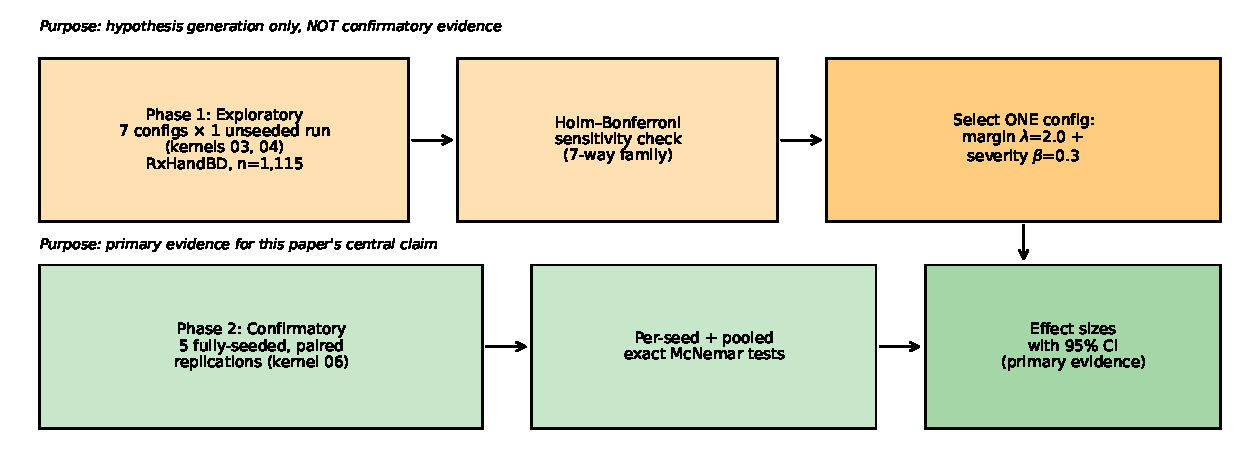
\includegraphics[width=0.85\textwidth]{figures/fig5_two_phase_design.pdf}
\caption{Overview of the two-phase exploratory/confirmatory experimental design. Phase 1 uses single, unseeded runs across many configurations purely to select one candidate; Phase 2 fully seeds and replicates only that one candidate, five times, each paired against a matched CE-only baseline retrained from the same seed.}
\label{fig:two-phase-design}
\end{figure}

\subsubsection*{Phase 1 --- exploratory ablation and hyperparameter sweep (kernels 03, 04)}\label{sec:phase1}

Phase 1's purpose is hypothesis generation and the \textbf{selection of a single candidate configuration} to carry forward to confirmatory testing. It is explicitly \textbf{not} intended, and not valid, as standalone confirmatory evidence, for two compounding reasons: (i) each configuration in Phase 1 was trained and evaluated only once, and (ii) training was not fully reproducibly seeded --- only Python's \texttt{random.seed} was set, while \texttt{torch} and \texttt{numpy} RNGs were left unseeded and \texttt{cudnn} was not set to deterministic mode. All Phase 1 comparisons use RxHandBD's single, fixed, 1,115-image test split.

Notably, even before any loss-design intervention, the fixed CE-only baseline used throughout Phase 1 (83/1,115 = 7.44\% \texttt{confusable\_wrong\_drug}; 519/1,115 = 46.5\% \texttt{correct}; 241/1,115 = 21.6\% \texttt{hallucination\_far\_off}) was itself one of two independent single CE-only fine-tuning runs on RxHandBD. A separate, earlier single CE-only run gave 81/1,115 = 7.26\% \texttt{confusable\_wrong\_drug}, 520/1,115 = 46.64\% \texttt{correct}, and 247/1,115 = 22.15\% \texttt{hallucination\_far\_off} --- consistent with the Phase 1 baseline within ordinary run-to-run noise. This run-to-run variability, present even in the absence of any loss-design change, is itself part of the motivation for the fully seeded, multi-run, paired confirmatory design of Phase 2 (\nameref{sec:phase2}).

\textbf{Batch (a) --- kernel 03} (\texttt{λ\_margin\ =\ 1.0} fixed), compared against the kernel-03 CE-only baseline (\texttt{confusable\_wrong\_drug} = 83/1,115 = 7.44\%):

\textbf{Table 4. Phase 1, batch (a) --- kernel 03 (single run per row, uncorrected p-values).}

\begin{longtable}[]{@{}
  >{\raggedright\arraybackslash}p{(\linewidth - 4\tabcolsep) * \real{0.3333}}
  >{\raggedright\arraybackslash}p{(\linewidth - 4\tabcolsep) * \real{0.3333}}
  >{\raggedright\arraybackslash}p{(\linewidth - 4\tabcolsep) * \real{0.3333}}@{}}
\toprule\noalign{}
\begin{minipage}[b]{\linewidth}\raggedright
Configuration
\end{minipage} & \begin{minipage}[b]{\linewidth}\raggedright
confusable\_wrong\_drug
\end{minipage} & \begin{minipage}[b]{\linewidth}\raggedright
p (uncorrected)
\end{minipage} \\
\midrule\noalign{}
\endhead
\bottomrule\noalign{}
\endlastfoot
CE-only baseline & 83/1,115 (7.44\%) & --- \\
Severity-only (β not tuned) & 88/1,115 (7.89\%) & 0.47 \\
Margin-only & 74/1,115 (6.64\%) & 0.18 \\
Severity + margin combined (kernel-03 defaults) & 83/1,115 (7.44\%) & 1.00 \\
\end{longtable}

Severity-only weighting alone did not help, and directionally slightly hurt --- an informative \emph{negative} finding, since up-weighting the loss for ``risky'' classes does not by itself teach the model to avoid one specific wrong answer. Margin-only was the only directionally positive signal in this batch. Severity and margin combined at their kernel-03 defaults returned to baseline, suggesting severity weighting can dilute margin's more targeted signal when combined naively at that weighting level.

\textbf{Batch (b) --- kernel 04 sweep}, all compared against the same fixed CE-only baseline (\texttt{confusable\_wrong\_drug} = 83/1,115 = 7.44\%; \texttt{correct} = 519/1,115 = 46.5\%; \texttt{hallucination\_far\_off} = 241/1,115 = 21.6\%):

\textbf{Table 5. Phase 1, batch (b) --- kernel 04 sweep (single run per row, uncorrected p-values).}

\begin{longtable}[]{@{}
  >{\raggedright\arraybackslash}p{(\linewidth - 6\tabcolsep) * \real{0.2500}}
  >{\raggedright\arraybackslash}p{(\linewidth - 6\tabcolsep) * \real{0.2500}}
  >{\raggedright\arraybackslash}p{(\linewidth - 6\tabcolsep) * \real{0.2500}}
  >{\raggedright\arraybackslash}p{(\linewidth - 6\tabcolsep) * \real{0.2500}}@{}}
\toprule\noalign{}
\begin{minipage}[b]{\linewidth}\raggedright
Configuration
\end{minipage} & \begin{minipage}[b]{\linewidth}\raggedright
confusable\_wrong\_drug (p)
\end{minipage} & \begin{minipage}[b]{\linewidth}\raggedright
correct (p)
\end{minipage} & \begin{minipage}[b]{\linewidth}\raggedright
hallucination\_far\_off (p)
\end{minipage} \\
\midrule\noalign{}
\endhead
\bottomrule\noalign{}
\endlastfoot
λ\_margin = 2.0 & 67/1,115, 6.01\% (0.009) & 44.0\% (0.014) & 24.3\% (0.0035) \\
λ\_margin = 3.0 & 59/1,115, 5.29\% (0.0001) & 44.4\% (0.021) & 24.5\% (0.0022) \\
λ\_margin = 2.0, 5 epochs (vs.\ 3) & 73/1,115, 6.55\% (0.14, n.s.) & 47.3\% (0.49, n.s.) & 22.0\% (0.75, n.s.) \\
λ\_margin = 2.0 + low severity β = 0.3 & 67/1,115, 6.01\% (0.011) & 523/1,115, 46.9\% (0.76, n.s.) & 250/1,115, 22.4\% (0.41, n.s.) \\
\end{longtable}

\texttt{λ\_margin\ =\ 3.0} gave the single largest raw reduction in \texttt{confusable\_wrong\_drug} found in Phase 1, but at a significant single-run cost to both \texttt{correct} and \texttt{hallucination\_far\_off}. The margin effect faded with longer training (5 vs.\ 3 epochs), consistent with CE eventually dominating the margin term. The configuration \textbf{λ\_margin = 2.0 + low severity β = 0.3} (β reduced roughly 3× from the kernel-03 default, not dropped entirely), trained for 3 epochs, was \textbf{selected} at the end of Phase 1 as the sole candidate carried forward to Phase 2, because in this single run it appeared to reduce the dangerous error category without a statistically significant single-run cost to \texttt{correct} or \texttt{hallucination\_far\_off}. As shown in \nameref{sec:phase2} below, this apparent cost-free benefit was a favorable statistical outlier rather than a robust property of the configuration.

\textbf{Multiple-comparisons sensitivity check.} A Holm--Bonferroni correction (\texttt{scripts/multiple\_comparisons.py}) was applied post hoc across the family of these seven Phase-1 single-run comparisons against the same CE-only baseline on the same RxHandBD test split, as a sensitivity/motivation check --- \textbf{not} as confirmatory evidence:

\textbf{Table 6. Holm--Bonferroni-adjusted results for selected Phase-1 comparisons.}

\begin{longtable}[]{@{}
  >{\raggedright\arraybackslash}p{(\linewidth - 6\tabcolsep) * \real{0.2500}}
  >{\raggedright\arraybackslash}p{(\linewidth - 6\tabcolsep) * \real{0.2500}}
  >{\raggedright\arraybackslash}p{(\linewidth - 6\tabcolsep) * \real{0.2500}}
  >{\raggedright\arraybackslash}p{(\linewidth - 6\tabcolsep) * \real{0.2500}}@{}}
\toprule\noalign{}
\begin{minipage}[b]{\linewidth}\raggedright
Configuration
\end{minipage} & \begin{minipage}[b]{\linewidth}\raggedright
p (uncorrected)
\end{minipage} & \begin{minipage}[b]{\linewidth}\raggedright
p (Holm--Bonferroni)
\end{minipage} & \begin{minipage}[b]{\linewidth}\raggedright
Survives at α = 0.05?
\end{minipage} \\
\midrule\noalign{}
\endhead
\bottomrule\noalign{}
\endlastfoot
λ\_margin = 3.0 & 0.0001 & 0.0008 & \textbf{Yes} \\
λ\_margin = 2.0 (alone) & 0.009 & 0.054 & No \\
λ\_margin = 2.0 + severity β = 0.3 (\textbf{selected}) & 0.011 & 0.057 & No \\
λ\_margin = 2.0, 5 epochs & 0.143 & 0.573 & No \\
λ\_margin = 1.0 (margin-only, kernel 03) & 0.176 & 0.573 & No \\
Severity-only, β not tuned (kernel 03) & 0.473 & 0.946 & No \\
Severity + margin combined, kernel-03 defaults & 1.000 & 1.000 & No \\
\end{longtable}

Critically, the configuration ultimately selected for Phase 2 does \textbf{not} survive this correction. This result is the explicit motivation for Phase 2: it demonstrates that none of the Phase 1 single-run findings --- including the one eventually selected --- can be trusted as final evidence on their own, given the researcher-degrees-of-freedom inherent in comparing many configurations on one fixed test set with unseeded single runs.

\begin{figure}[htbp]
\centering
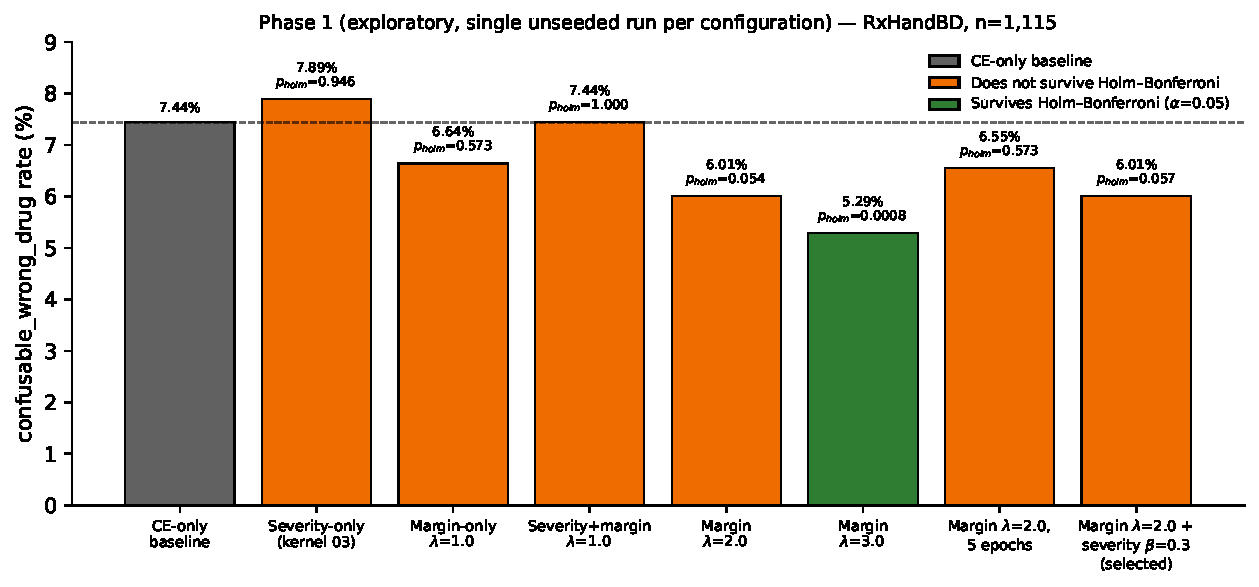
\includegraphics[width=0.9\textwidth]{figures/fig2_phase1_exploratory_sweep.pdf}
\caption{Phase 1 exploratory hyperparameter sweep (kernel 04): confusable\_wrong\_drug rate against the fixed CE-only baseline, single unseeded run per configuration. Uncorrected p-values are shown above each bar; only $\lambda_{\text{margin}}=3.0$ survives Holm--Bonferroni correction (Table 6), and the selected configuration ($\lambda_{\text{margin}}=2.0$ + severity $\beta=0.3$) does not.}
\label{fig:phase1-sweep}
\end{figure}

\textbf{Cross-dataset check (kernel 05).} The Phase-1-selected configuration was additionally applied, in a single run, to Kaggle-BD. It did not replicate: \texttt{confusable\_wrong\_drug} moved from 3/780 (0.38\%) to 4/780 (0.51\%) (p = 1.00, uninformative given only 3--4 affected images), while the \texttt{correct} rate significantly \emph{decreased} (87.7\% → 86.0\%, p = 0.041) with no measurable compensating benefit, and \texttt{hallucination\_far\_off} was unchanged (p = 0.26). The most likely interpretation is that the intervention needs a large, LASA-rich vocabulary to have ``room'' to act; on a small, closed, 78-class vocabulary already close to saturated performance, it mostly adds training noise. Accordingly, this study's confirmed claims (\nameref{sec:phase2}) are scoped to RxHandBD-like settings --- larger, more LASA-dense, open vocabularies --- and are not claimed to generalize to arbitrary handwritten drug-name OCR settings.

\subsubsection*{Phase 2 --- confirmatory replication (kernel 06)}\label{sec:phase2}

Phase 2 constitutes this paper's primary evidence. The single Phase-1-selected configuration (λ\_margin = 2.0 + severity β = 0.3, 3 epochs) was retrained from scratch \textbf{five times}, each with a different, \textbf{fully seeded} random seed: Python's \texttt{random}, NumPy, and both \texttt{torch} and \texttt{torch.cuda} RNGs were all seeded, with \texttt{cudnn.deterministic\ =\ True}, \texttt{cudnn.benchmark\ =\ False}, and \texttt{DataLoader\ num\_workers\ =\ 0} for determinism.

Each of the five seeded runs of the winning configuration is \textbf{paired} against a CE-only baseline retrained with the \emph{same} seed, reset immediately before that baseline's own training begins. This pairing design is what isolates the loss-function effect from other sources of run-to-run variation: because the seed governing LoRA weight initialization and data-shuffle order is identical within each pair, any systematic difference between the two arms of a pair is attributable to the change in loss function, not to initialization or shuffling noise. All five seed-pairs are evaluated on the same fixed RxHandBD 1,115-image test split used throughout this study.

\textbf{Statistical testing.} Per-seed and pooled significance are assessed with paired, \textbf{exact} McNemar tests, computed as \texttt{scipy.stats.binomtest} applied to the discordant pairs between the two arms of each comparison --- never the approximate/chi-square McNemar approximation, following the paired-significance-testing protocol argued for by \citet{dror2018hitchhikers}. Effect sizes for the pooled analysis are reported with 95\% confidence intervals using a Wald interval for the difference of two \textbf{paired} proportions (\texttt{scripts/analyze\_confirmatory\_extended.py}):

\begin{quote}
\texttt{d = $p_{01}$ $-$ $p_{10}$}\\
\texttt{Var(d) = [$p_{10}$ + $p_{01}$ $-$ ($p_{01}$ $-$ $p_{10}$)$^2$] / n}
\end{quote}

evaluated on the pooled n = 5,575 paired comparisons (5 seeds × 1,115 test images). Full per-seed and pooled results, effect sizes, and the associated destination-of-error and overcorrection analyses are reported in the Results section.

\subsubsection*{Two-phase design as a reusable template}\label{sec:two-phase-template}

Beyond its role in this specific study, the exploratory/confirmatory structure described above --- an unseeded, single-run hyperparameter sweep used only for hypothesis generation and configuration selection, combined with a Holm--Bonferroni sensitivity check on that sweep, followed by a small number of fully seeded, paired-by-seed confirmatory replications with exact paired significance testing --- is proposed as a reusable template for similarly small-scale OCR safety studies, where full-scale multi-seed replication of every candidate configuration is computationally impractical but a single-run sweep alone is not a credible basis for a final claim, for the reasons documented across the reproducibility literature reviewed in \nameref{sec:related-repro}.

\section*{Results}\label{sec:results}

\subsection*{Phase 0: Reproduction of the Motivating Phenomenon}\label{sec:phase0-results}

Before any loss-function intervention, both datasets were evaluated with zero-shot pretrained TrOCR (\texttt{microsoft/trocr-base-handwritten}) and with a single-run, CE-only LoRA fine-tune (r=16, α=32, dropout=0.05, target modules \texttt{[q\_proj,\ v\_proj]}, bias=\texttt{none}, peft 0.13.2, 3 epochs, batch size 8, lr=1e-4). A classical OCR engine (Tesseract) was also benchmarked zero-shot as a reference point on RxHandBD and performed far worse than TrOCR on handwritten drug names (correct rate: Tesseract 4.30\% vs.\ TrOCR 19.55\%); Tesseract was therefore not carried forward, and TrOCR was used as the sole fine-tuning backbone for the remainder of the study.

\textbf{Table 7.} Zero-shot vs.\ single-run CE-only LoRA fine-tuning, by dataset and error category.

\begin{longtable}[]{@{}
  >{\raggedright\arraybackslash}p{(\linewidth - 8\tabcolsep) * \real{0.2000}}
  >{\raggedright\arraybackslash}p{(\linewidth - 8\tabcolsep) * \real{0.2000}}
  >{\raggedright\arraybackslash}p{(\linewidth - 8\tabcolsep) * \real{0.2000}}
  >{\raggedright\arraybackslash}p{(\linewidth - 8\tabcolsep) * \real{0.2000}}
  >{\raggedright\arraybackslash}p{(\linewidth - 8\tabcolsep) * \real{0.2000}}@{}}
\toprule\noalign{}
\begin{minipage}[b]{\linewidth}\raggedright
Dataset
\end{minipage} & \begin{minipage}[b]{\linewidth}\raggedright
Configuration
\end{minipage} & \begin{minipage}[b]{\linewidth}\raggedright
Correct
\end{minipage} & \begin{minipage}[b]{\linewidth}\raggedright
Hallucination (far-off)
\end{minipage} & \begin{minipage}[b]{\linewidth}\raggedright
Confusable (wrong drug)
\end{minipage} \\
\midrule\noalign{}
\endhead
\bottomrule\noalign{}
\endlastfoot
Kaggle-BD (n=780, 78-class) & Zero-shot TrOCR & 22.95\% (179/780) & 60.77\% (474/780) & 0.38\% (3/780) \\
Kaggle-BD (n=780, 78-class) & LoRA CE-only fine-tune & 87.95\% (686/780) & 5.77\% (45/780) & 0.64\% (5/780) \\
RxHandBD (n=1115, \textasciitilde1430 label instances) & Zero-shot TrOCR & 19.55\% (218/1115) & 60.90\% (679/1115) & 1.79\% (20/1115) \\
RxHandBD (n=1115, \textasciitilde1430 label instances) & LoRA CE-only fine-tune (Run 1) & 46.64\% (520/1115) & 22.15\% (247/1115) & 7.26\% (81/1115) \\
\end{longtable}

A second, independently-trained CE-only run on RxHandBD gave confusable\_wrong\_drug = 83/1115 (7.44\%), correct = 519/1115 (46.5\%), hallucination\_far\_off = 241/1115 (21.6\%) --- consistent with Run 1 within expected run-to-run noise. This second run is reused as the fixed reference baseline for the exploratory ablation/sweep phase (\nameref{sec:phase1-results}), and the run-to-run variability observed here is precisely what later motivated the fully-seeded, multi-run confirmatory design of Phase 2 (\nameref{sec:phase2-results}).

\textbf{Interpretation.} On both datasets, LoRA fine-tuning produces a large overall improvement: hallucination\_far\_off drops sharply and correct rate rises substantially. On the small, closed-vocabulary Kaggle-BD dataset (78 classes), the dangerous confusable\_wrong\_drug category remains negligible after fine-tuning (3→5 images out of 780; not a meaningful signal on its own). On the larger, more LASA-rich RxHandBD vocabulary, however, the same fine-tuning procedure that drives the large overall gains also increases confusable\_wrong\_drug by roughly 4× in relative terms (1.79\% → \textasciitilde7.3\%). This is the motivating paradox for the present study --- overall accuracy improves sharply while the single most clinically dangerous error type gets worse --- and it is most pronounced on RxHandBD, independently reproducing the prior project's finding \citep{dang2026zeroshot} on new public data, a new codebase, and new labels.

\begin{figure}[htbp]
\centering
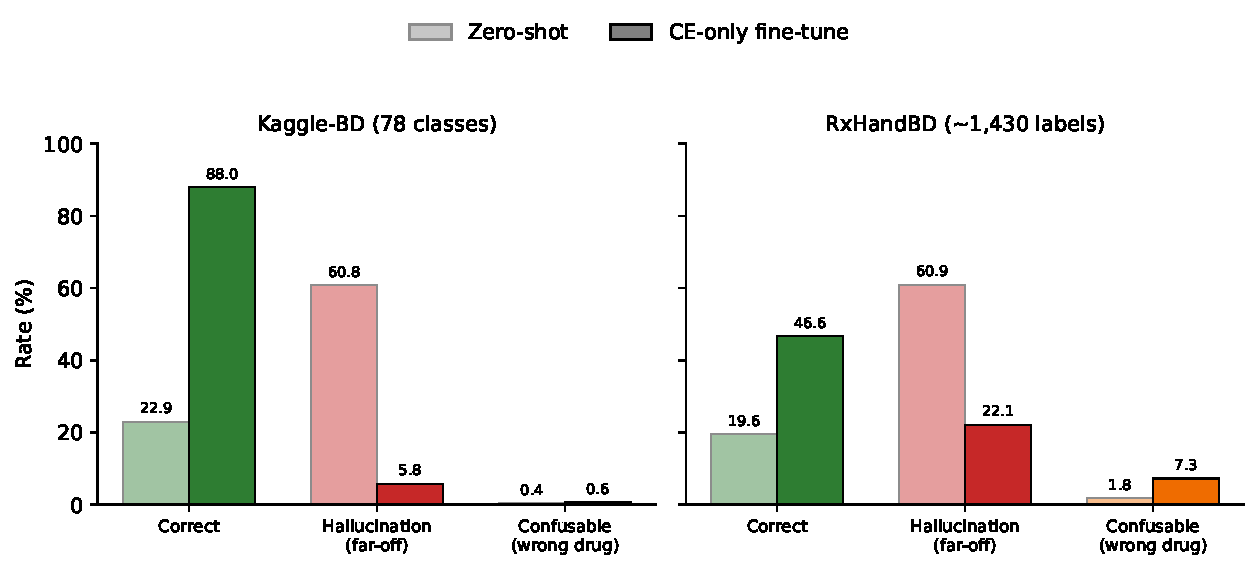
\includegraphics[width=0.95\textwidth]{figures/fig1_phase0_zeroshot_vs_finetune.pdf}
\caption{Zero-shot versus single-run CE-only LoRA fine-tuning, by dataset and error category (Table 7). Fine-tuning improves correct rate and collapses hallucination on both datasets, but only RxHandBD shows a corresponding rise in the dangerous confusable\_wrong\_drug category.}
\label{fig:phase0}
\end{figure}

\subsection*{Phase 1: Exploratory Ablation and Hyperparameter Sweep}\label{sec:phase1-results}

\textbf{This subsection is exploratory and hypothesis-generating only.} Each configuration below was trained and evaluated exactly once, without full RNG seeding (only Python's \texttt{random.seed} was set; PyTorch and NumPy generators were not seeded, and cuDNN was not set to deterministic mode), on RxHandBD's single fixed 1115-image test split. None of the p-values in this subsection are corrected for the multiple configurations compared, and none should be read as confirmed statistical significance --- a caveat consistent with the general single-run pitfalls documented in \nameref{sec:related-repro}; Phase 1's sole purpose is to select one candidate configuration for confirmatory replication in Phase 2.

All comparisons in this subsection are against the same CE-only baseline (Run 2 from \nameref{sec:phase0-results}): confusable\_wrong\_drug = 83/1115 (7.44\%), correct = 519/1115 (46.5\%), hallucination\_far\_off = 241/1115 (21.6\%).

\textbf{Kernel 03 --- fixed λ\_margin = 1.0, varying loss components} (confusable\_wrong\_drug only; p-values uncorrected, single run):

\textbf{Table 8.} Kernel 03 ablation batch.

\begin{longtable}[]{@{}
  >{\raggedright\arraybackslash}p{(\linewidth - 4\tabcolsep) * \real{0.3333}}
  >{\raggedright\arraybackslash}p{(\linewidth - 4\tabcolsep) * \real{0.3333}}
  >{\raggedright\arraybackslash}p{(\linewidth - 4\tabcolsep) * \real{0.3333}}@{}}
\toprule\noalign{}
\begin{minipage}[b]{\linewidth}\raggedright
Configuration
\end{minipage} & \begin{minipage}[b]{\linewidth}\raggedright
Confusable (wrong drug)
\end{minipage} & \begin{minipage}[b]{\linewidth}\raggedright
p (uncorrected)
\end{minipage} \\
\midrule\noalign{}
\endhead
\bottomrule\noalign{}
\endlastfoot
CE-only baseline & 83/1115 (7.44\%) & --- \\
Severity-only (β not tuned) & 88/1115 (7.89\%) & 0.47 \\
Margin-only & 74/1115 (6.64\%) & 0.18 \\
Severity + margin combined (kernel-03 defaults) & 83/1115 (7.44\%) & 1.00 \\
\end{longtable}

Severity-only is directionally \emph{worse} than baseline; margin-only is the single directionally-positive signal in this batch; severity+margin combined returns to baseline, suggesting severity weighting dilutes margin's targeted signal when combined naively at these settings.

\textbf{Kernel 04 --- sweep over margin λ, training length, and low-β severity:}

\textbf{Table 9.} Kernel 04 sweep, all vs.\ the CE-only baseline above (uncorrected, single run).

\begin{longtable}[]{@{}
  >{\raggedright\arraybackslash}p{(\linewidth - 6\tabcolsep) * \real{0.2500}}
  >{\raggedright\arraybackslash}p{(\linewidth - 6\tabcolsep) * \real{0.2500}}
  >{\raggedright\arraybackslash}p{(\linewidth - 6\tabcolsep) * \real{0.2500}}
  >{\raggedright\arraybackslash}p{(\linewidth - 6\tabcolsep) * \real{0.2500}}@{}}
\toprule\noalign{}
\begin{minipage}[b]{\linewidth}\raggedright
Configuration
\end{minipage} & \begin{minipage}[b]{\linewidth}\raggedright
Confusable (wrong drug), p
\end{minipage} & \begin{minipage}[b]{\linewidth}\raggedright
Correct, p
\end{minipage} & \begin{minipage}[b]{\linewidth}\raggedright
Hallucination (far-off), p
\end{minipage} \\
\midrule\noalign{}
\endhead
\bottomrule\noalign{}
\endlastfoot
CE-only baseline & 83/1115 (7.44\%) & 519/1115 (46.5\%) & 241/1115 (21.6\%) \\
Margin λ=2.0 (3 epochs) & 67/1115 (6.01\%), p=0.009 & 44.0\%, p=0.014 & 24.3\%, p=0.0035 \\
Margin λ=3.0 (3 epochs) & 59/1115 (5.29\%), p=0.0001 & 44.4\%, p=0.021 & 24.5\%, p=0.0022 \\
Margin λ=2.0, 5 epochs & 73/1115 (6.55\%), p=0.14 (NS) & 527/1115, 47.3\%, p=0.49 (NS) & 245/1115, 22.0\%, p=0.75 (NS) \\
\textbf{Margin λ=2.0 + severity β=0.3 (selected)} & 67/1115 (6.01\%), p=0.011 & 523/1115 (46.9\%), p=0.76 (NS) & 250/1115 (22.4\%), p=0.41 (NS) \\
\end{longtable}

Margin λ=3.0 gives the single largest raw reduction in confusable\_wrong\_drug found in Phase 1, but at significant single-run costs to correct rate and hallucination rate. Extending margin λ=2.0 training from 3 to 5 epochs erodes the confusable-rate effect (p=0.14), suggesting the CE term eventually dominates the margin term with longer training. The configuration \textbf{margin λ=2.0 + severity β=0.3} (β reduced \textasciitilde3× from the kernel-03 default, not dropped) was selected at the end of Phase 1 as the sole candidate carried forward to Phase 2, because in this single run it appeared to reduce the dangerous error category without a statistically significant single-run cost to correct rate or hallucination rate. As shown in \nameref{sec:phase2-results}, this apparent ``free lunch'' was a favorable statistical outlier rather than a real property of the configuration.

\textbf{Holm-Bonferroni sensitivity check.} A Holm-Bonferroni correction (\texttt{scripts/multiple\_comparisons.py}) was applied post hoc across the family of the 7 Phase-1 single-run comparisons above (all vs.\ the same CE-only baseline, same RxHandBD split), as a sensitivity/motivation check --- not as confirmatory evidence, in the spirit of the significance-testing protocol recommended by \citet{dror2018hitchhikers}.

\textbf{Table 10.} Holm-Bonferroni outcome for the 7 Phase-1 configurations (confusable\_wrong\_drug metric).

\begin{longtable}[]{@{}
  >{\raggedright\arraybackslash}p{(\linewidth - 6\tabcolsep) * \real{0.2500}}
  >{\raggedright\arraybackslash}p{(\linewidth - 6\tabcolsep) * \real{0.2500}}
  >{\raggedright\arraybackslash}p{(\linewidth - 6\tabcolsep) * \real{0.2500}}
  >{\raggedright\arraybackslash}p{(\linewidth - 6\tabcolsep) * \real{0.2500}}@{}}
\toprule\noalign{}
\begin{minipage}[b]{\linewidth}\raggedright
Configuration
\end{minipage} & \begin{minipage}[b]{\linewidth}\raggedright
Uncorrected p
\end{minipage} & \begin{minipage}[b]{\linewidth}\raggedright
p (Holm-Bonferroni)
\end{minipage} & \begin{minipage}[b]{\linewidth}\raggedright
Survives at α=0.05?
\end{minipage} \\
\midrule\noalign{}
\endhead
\bottomrule\noalign{}
\endlastfoot
Kernel 03: severity-only & 0.473 & 0.946 & No \\
Kernel 03: margin-only & 0.176 & 0.573 & No \\
Kernel 03: severity+margin combined & 1.000 & 1.000 & No \\
Kernel 04: margin λ=2.0 & 0.009 & 0.054 & No \\
Kernel 04: margin λ=3.0 & 0.0001 & 0.0008 & \textbf{Yes} \\
Kernel 04: margin λ=2.0, 5 epochs & 0.143 & 0.573 & No \\
Kernel 04: margin λ=2.0 + severity β=0.3 (selected) & 0.011 & 0.057 & No \\
\end{longtable}

\textbf{Stated conclusion.} Only ``margin λ=3.0'' survives Holm-Bonferroni correction; critically, the configuration actually selected for Phase 2 (``margin λ=2.0 + severity β=0.3'') does \emph{not} survive (p\_holm=0.057), nor does ``margin λ=2.0'' alone (p\_holm=0.054). This result is the explicit motivation for Phase 2: it demonstrates that none of the Phase-1 single-run findings --- including the one eventually selected --- can be trusted as final evidence on their own, given the researcher-degrees-of-freedom inherent in comparing many configurations on one fixed test set with unseeded single runs.

\subsection*{Cross-Dataset Check (Kaggle-BD Non-Replication)}\label{sec:cross-dataset-check}

The Phase-1-selected configuration (margin λ=2.0 + severity β=0.3) was applied, in a single run, to Kaggle-BD (kernel 05).

\textbf{Table 11.} Cross-dataset check on Kaggle-BD (CE-only baseline vs.\ selected configuration).

\begin{longtable}[]{@{}
  >{\raggedright\arraybackslash}p{(\linewidth - 8\tabcolsep) * \real{0.2000}}
  >{\raggedright\arraybackslash}p{(\linewidth - 8\tabcolsep) * \real{0.2000}}
  >{\raggedright\arraybackslash}p{(\linewidth - 8\tabcolsep) * \real{0.2000}}
  >{\raggedright\arraybackslash}p{(\linewidth - 8\tabcolsep) * \real{0.2000}}
  >{\raggedright\arraybackslash}p{(\linewidth - 8\tabcolsep) * \real{0.2000}}@{}}
\toprule\noalign{}
\begin{minipage}[b]{\linewidth}\raggedright
Metric
\end{minipage} & \begin{minipage}[b]{\linewidth}\raggedright
CE-only baseline
\end{minipage} & \begin{minipage}[b]{\linewidth}\raggedright
Selected configuration
\end{minipage} & \begin{minipage}[b]{\linewidth}\raggedright
p-value
\end{minipage} & \begin{minipage}[b]{\linewidth}\raggedright
Note
\end{minipage} \\
\midrule\noalign{}
\endhead
\bottomrule\noalign{}
\endlastfoot
Confusable (wrong drug) & 3/780 (0.38\%) & 4/780 (0.51\%) & 1.00 & Uninformative given only 3--4 affected images \\
Correct & 87.7\% & 86.0\% & 0.041 & Significant decrease \\
Hallucination (far-off) & --- & --- & 0.26 & Unchanged \\
\end{longtable}

\textbf{Interpretation.} The Phase-1-selected configuration did not replicate on Kaggle-BD: the confusable\_wrong\_drug change is statistically uninformative given the tiny number of affected images, while correct rate significantly \emph{decreased} with no measurable compensating benefit, and hallucination rate was unchanged. This is consistent with the intervention needing a large, LASA-rich vocabulary to have ``room'' to help; on a small, closed 78-class vocabulary already close to saturated performance, it mostly adds training noise. Accordingly, the paper's confirmed claims (\nameref{sec:phase2-results}) are scoped to RxHandBD-like settings --- larger, more LASA-dense, open vocabularies --- and are not claimed to generalize to arbitrary handwritten drug-name OCR settings.

\subsection*{Phase 2: Confirmatory Replication (Primary Evidence)}\label{sec:phase2-results}

The single Phase-1-selected configuration (margin λ=2.0 + severity β=0.3, 3 epochs --- ``the winning configuration'') was retrained from scratch 5 times with 5 different, fully seeded random seeds (Python \texttt{random}, NumPy, and PyTorch/CUDA RNGs all seeded; \texttt{cudnn.deterministic=True}, \texttt{cudnn.benchmark=False}; \texttt{DataLoader(num\_workers=0)}), each paired against a CE-only baseline retrained with the same seed reset immediately before that baseline's own training --- isolating the loss-function effect from LoRA-initialization and data-shuffle-order noise. All 5 seed-pairs were evaluated on the same fixed RxHandBD 1115-image test split. Per-seed and pooled paired McNemar exact tests (\texttt{scipy.stats.binomtest} on discordant pairs) were used throughout --- never an approximate/chi-square McNemar test.

\textbf{Table 12.} Per-seed results, CE-only → winning configuration (exact McNemar p-values).

\begin{longtable}[]{@{}llll@{}}
\toprule\noalign{}
Seed & Confusable (wrong drug) & Correct & Hallucination (far-off) \\
\midrule\noalign{}
\endhead
\bottomrule\noalign{}
\endlastfoot
1 & 79 → 65 (p=0.049) & 522 → 495 (p=0.011) & 242 → 268 (p=0.018) \\
2 & 74 → 68 (p=0.362) & 524 → 508 (p=0.101) & 238 → 275 (p=0.0002) \\
3 & 90 → 79 (p=0.043) & 513 → 503 (p=0.368) & 238 → 254 (p=0.109) \\
4 & 78 → 66 (p=0.036) & 526 → 498 (p=0.010) & 235 → 255 (p=0.045) \\
5 & 78 → 71 (p=0.265) & 529 → 498 (p=0.005) & 243 → 264 (p=0.033) \\
\end{longtable}

All three metrics move in the \textbf{same direction in all 5/5 seeds, with no exceptions}: confusable\_wrong\_drug always decreases, correct always decreases, hallucination\_far\_off always increases.

\textbf{Table 13.} Pooled results across 5 seeds (n=5,575 paired comparisons; one pooled exact McNemar test per metric).

\begin{longtable}[]{@{}
  >{\raggedright\arraybackslash}p{(\linewidth - 8\tabcolsep) * \real{0.2000}}
  >{\raggedright\arraybackslash}p{(\linewidth - 8\tabcolsep) * \real{0.2000}}
  >{\raggedright\arraybackslash}p{(\linewidth - 8\tabcolsep) * \real{0.2000}}
  >{\raggedright\arraybackslash}p{(\linewidth - 8\tabcolsep) * \real{0.2000}}
  >{\raggedright\arraybackslash}p{(\linewidth - 8\tabcolsep) * \real{0.2000}}@{}}
\toprule\noalign{}
\begin{minipage}[b]{\linewidth}\raggedright
Metric
\end{minipage} & \begin{minipage}[b]{\linewidth}\raggedright
Discordant pairs (favor CE-only / favor winning)
\end{minipage} & \begin{minipage}[b]{\linewidth}\raggedright
Pooled p
\end{minipage} & \begin{minipage}[b]{\linewidth}\raggedright
Mean rate, CE-only → winning
\end{minipage} & \begin{minipage}[b]{\linewidth}\raggedright
Individually significant seeds (p\textless0.05)
\end{minipage} \\
\midrule\noalign{}
\endhead
\bottomrule\noalign{}
\endlastfoot
Confusable (wrong drug) & 103 fixed / 53 newly & 0.000077 & 7.16\% → 6.26\% (relative reduction \textasciitilde12.6\%) & 3/5 \\
Correct & 312 lost / 200 gained & 0.000001 & 46.9\% → 44.9\% (absolute drop \textasciitilde2.0 points) & 3/5 \\
Hallucination (far-off) & 178 lost / 298 gained & \textless0.000001 & 21.5\% → 23.6\% (absolute rise \textasciitilde2.2 points) & 4/5 \\
\end{longtable}

\textbf{Table 14.} Effect sizes with 95\% CI for paired proportions (Wald CI, pooled n=5,575; \texttt{scripts/analyze\_confirmatory\_extended.py}).

\begin{longtable}[]{@{}lll@{}}
\toprule\noalign{}
Metric & Risk difference (percentage points) & 95\% CI \\
\midrule\noalign{}
\endhead
\bottomrule\noalign{}
\endlastfoot
Confusable (wrong drug) & −0.90 & [−1.34, −0.46] \\
Correct & −2.01 & [−2.80, −1.22] \\
Hallucination (far-off) & +2.15 & [+1.39, +2.92] \\
\end{longtable}

All three 95\% CIs exclude zero, consistent with the pooled p-values above.

\begin{figure}[htbp]
\centering
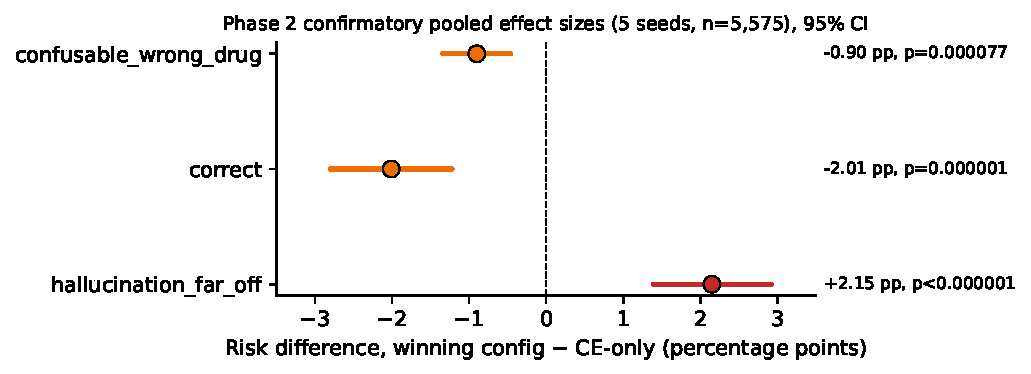
\includegraphics[width=0.8\textwidth]{figures/fig3_phase2_forest_plot.pdf}
\caption{Forest plot of the three pooled risk differences (Table 14) with 95\% Wald confidence intervals for paired proportions, n=5,575 pooled paired comparisons across 5 confirmatory seeds. All three intervals exclude zero.}
\label{fig:forest-plot}
\end{figure}

\textbf{Correction of the earlier single-run impression.} The Phase-1 single run for this exact configuration (Table 9, \nameref{sec:phase1-results}) reported correct = 46.9\% (p=0.76, not significant) and hallucination\_far\_off = 22.4\% (p=0.41, not significant) alongside the confusable-rate reduction, creating an impression that the dangerous error type could be reduced ``without a significant cost.'' The 5-seed Phase-2 confirmatory replication corrects this impression: pooled effects on all three metrics are statistically robust (Table 13, Table 14), with correct rate significantly \emph{decreasing} and hallucination rate significantly \emph{increasing} --- not neutral, as the single Phase-1 run had suggested. The Phase-1 result was a favorable statistical outlier, not a real, cost-free property of the configuration --- an instructive real-world instance of exactly the single-run pitfall documented by \citet{henderson2018deep} and \citet{bouthillier2019unreproducible}. The robust, confirmed effect is that this loss combination fixes \textasciitilde12.6\% (relative) of the most dangerous error type at a real, statistically robust cost of \textasciitilde2.0 points of overall correct rate and \textasciitilde2.2 points of hallucination rate.

\subsection*{Safety-Oriented Secondary Analyses}\label{sec:safety-secondary}

\textbf{Destination of ``fixed'' confusable errors.} Pooled across all 5 seeds, CE-only produced 399 confusable\_wrong\_drug errors in total; of these, 103 (25.8\%) were no longer classified as confusable\_wrong\_drug under the winning configuration.

\textbf{Table 15.} Destination of the 103 resolved confusable\_wrong\_drug errors (pooled, 5 seeds).

\begin{longtable}[]{@{}lll@{}}
\toprule\noalign{}
Destination category & n (of 103) & Share \\
\midrule\noalign{}
\endhead
\bottomrule\noalign{}
\endlastfoot
Correct & 36 & 35.0\% \\
Minor OCR noise & 37 & --- \\
Hallucination (far-off) & 30 & --- \\
\textbf{Clearly wrong (minor noise + hallucination)} & \textbf{67} & \textbf{65.0\%} \\
\end{longtable}

\begin{figure}[htbp]
\centering
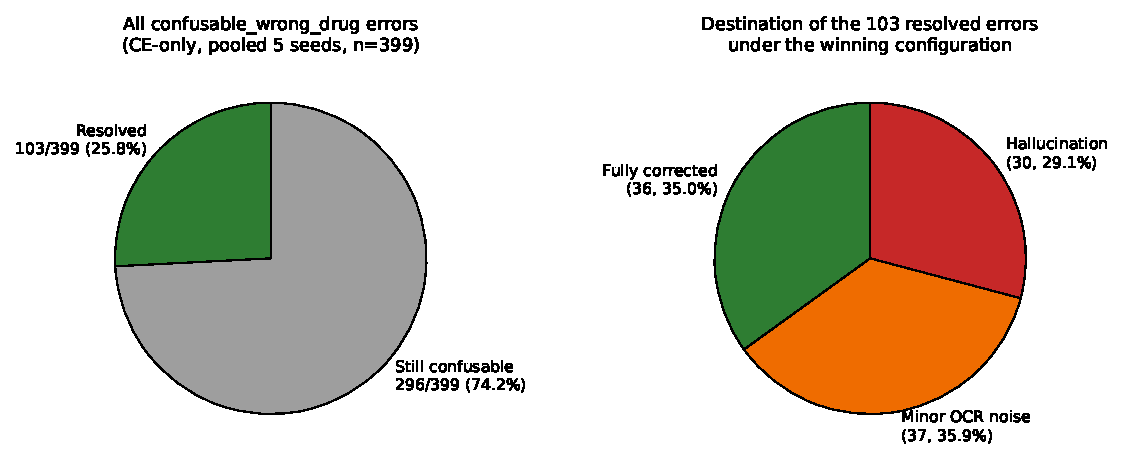
\includegraphics[width=0.75\textwidth]{figures/fig4_destination_breakdown.pdf}
\caption{Destination of the 103 resolved confusable\_wrong\_drug errors under the winning configuration, pooled across 5 seeds (Table 15). Most resolved dangerous errors (65.0\%) become an overtly wrong output rather than a correct one.}
\label{fig:destination}
\end{figure}

Only 35.0\% of resolved dangerous errors became fully correct; the majority (65.0\%) were converted into an obviously-wrong error type instead (minor\_ocr\_noise or hallucination\_far\_off) rather than into a correct reading. Clinically, an obviously-wrong output (e.g., a nonsense string) is far easier for a pharmacist or clinician to catch and query than a fluent, plausible but wrong real drug name --- so this destination shift represents a genuine safety benefit that the raw confusable\_wrong\_drug rate alone does not capture.

\textbf{Overcorrection (``new confusion'') check.} Pooled across the 5 seeds, of the images that were correct under CE-only, only 16/2,614 (0.61\%, Wilson 95\% CI [0.38\%, 0.99\%]) became \emph{newly} classified as confusable\_wrong\_drug under the winning configuration. Only a small minority of the \textasciitilde2-point overall correct-rate loss documented in \nameref{sec:phase2-results} is converted into the specific dangerous error type; most of the lost correct predictions instead become less-dangerous minor-noise or hallucination errors.

\textbf{Note on error categorization.} All counts above (correct / minor\_ocr\_noise / confusable\_wrong\_drug / other\_wrong\_real\_word / hallucination\_far\_off) are produced by the automated, threshold-based \texttt{classify\_error()} classifier (BI-SIM similarity to the true label and to the dataset vocabulary; CONFUSABLE\_THRESHOLD=0.65), not by human pharmacist adjudication of individual predictions. This is a modeling choice, not ground truth, and is treated as an explicit limitation of the study (see Limitations).

\section*{Discussion}\label{sec:discussion}

\subsection*{A quantified operating point, not a free improvement}\label{sec:disc-quantified}

The five-seed confirmatory replication (Phase 2) shows that the combined margin-ranking-plus-severity-weighted loss (λ\_margin = 2.0, β = 0.3) does not remove the confusable\_wrong\_drug problem at no cost. It instead defines one statistically robust point on a trade-off curve between the rate of dangerous look-alike, sound-alike (LASA) errors and overall recognition accuracy. Pooled across 5,575 paired predictions (five seeds × 1,115 RxHandBD test images), the confusable\_wrong\_drug rate fell from a mean of 7.16\% under CE-only training to 6.26\% under the winning configuration --- a 12.6\% relative reduction (pooled exact McNemar p = 0.000077; risk difference −0.90 points, 95\% CI [−1.34, −0.46]) --- while the overall correct rate fell from 46.9\% to 44.9\% (pooled p = 0.000001; risk difference −2.01 points, 95\% CI [−2.80, −1.22]) and the hallucination\_far\_off rate rose from 21.5\% to 23.6\% (pooled p \textless{} 0.000001; risk difference +2.15 points, 95\% CI [+1.39, +2.92]).

\begin{longtable}[]{@{}
  >{\raggedright\arraybackslash}p{(\linewidth - 10\tabcolsep) * \real{0.1667}}
  >{\raggedright\arraybackslash}p{(\linewidth - 10\tabcolsep) * \real{0.1667}}
  >{\raggedright\arraybackslash}p{(\linewidth - 10\tabcolsep) * \real{0.1667}}
  >{\raggedright\arraybackslash}p{(\linewidth - 10\tabcolsep) * \real{0.1667}}
  >{\raggedright\arraybackslash}p{(\linewidth - 10\tabcolsep) * \real{0.1667}}
  >{\raggedright\arraybackslash}p{(\linewidth - 10\tabcolsep) * \real{0.1667}}@{}}
\toprule\noalign{}
\begin{minipage}[b]{\linewidth}\raggedright
Metric
\end{minipage} & \begin{minipage}[b]{\linewidth}\raggedright
CE-only (mean)
\end{minipage} & \begin{minipage}[b]{\linewidth}\raggedright
Winning configuration (mean)
\end{minipage} & \begin{minipage}[b]{\linewidth}\raggedright
Pooled exact McNemar \emph{p}
\end{minipage} & \begin{minipage}[b]{\linewidth}\raggedright
Risk difference (pp)
\end{minipage} & \begin{minipage}[b]{\linewidth}\raggedright
95\% CI
\end{minipage} \\
\midrule\noalign{}
\endhead
\bottomrule\noalign{}
\endlastfoot
confusable\_wrong\_drug & 7.16\% & 6.26\% & 0.000077 & −0.90 & [−1.34, −0.46] \\
correct & 46.9\% & 44.9\% & 0.000001 & −2.01 & [−2.80, −1.22] \\
hallucination\_far\_off & 21.5\% & 23.6\% & \textless0.000001 & +2.15 & [+1.39, +2.92] \\
\end{longtable}

All three metrics moved in the same direction in every one of the five seeds, with no exceptions --- direction-consistent evidence for a real property of this loss combination rather than a single favorable run. That uniformity matters because the corresponding Phase-1 single run for this exact configuration reported changes in correct rate and hallucination rate that were not statistically significant (p = 0.76, p = 0.41), a result an earlier internal draft of this manuscript read as reducing the dangerous error ``without a significant cost.'' The confirmatory replication corrects that reading: the apparent absence of cost was a favorable statistical outlier in one unseeded run, not a property of the method. We therefore frame the contribution as a disclosed, measured operating point --- a roughly one-eighth relative reduction in the single most dangerous error category, purchased at a roughly two-point cost to raw accuracy and a roughly two-point increase in nonsense output --- rather than a strictly dominant improvement.

\subsection*{Where resolved dangerous errors go: a fail-safe interpretation}\label{sec:disc-failsafe}

Not all of the correct-rate loss carries equal clinical weight, because a real drug-name substitution and a nonsense string are not equally likely to be caught downstream. Of the 399 confusable\_wrong\_drug errors CE-only training produced across all five seeds, 103 (25.8\%) were no longer classified as confusable\_wrong\_drug under the winning configuration. Of those 103 resolved errors, only 36 (35.0\%) became fully correct; the remaining 67 (65.0\%) became minor\_ocr\_noise (37 cases) or hallucination\_far\_off (30 cases) --- outputs that do not resemble a plausible, valid drug name. A LASA substitution is dangerous precisely because it produces a fluent, plausible prescription that gives a pharmacist reading the output no obvious reason to double-check it; an overtly wrong string, by contrast, is the kind of failure a verification step is built to catch. On that basis, converting a LASA error into an overt error has downstream safety value that the raw correct/incorrect split does not capture, though this argument presumes a human verification step exists downstream and is not a claim that the system is safe to deploy without one.

\subsection*{Overcorrection is rare: the added cost is mostly safe in kind}\label{sec:disc-overcorrection}

The accuracy cost is also not concentrated in manufacturing new instances of the error type this study targets. Of images CE-only training got correct, only 16 of 2,614 (0.61\%, Wilson 95\% CI [0.38\%, 0.99\%]) became newly confusable\_wrong\_drug under the winning configuration; the rest of the lost correct predictions moved into minor\_ocr\_noise or hallucination\_far\_off. We describe this cost as mostly safe in kind: the roughly two-point drop in correct rate reported above is real and statistically robust, but it is largely not being converted into the one failure mode the intervention is designed to reduce. This qualifies the size of the trade-off without removing it.

\subsection*{A vocabulary-size hypothesis for the cross-dataset non-replication}\label{sec:disc-vocab}

The winning configuration did not replicate when applied, in a single run, to Kaggle-BD's 78-class closed vocabulary: confusable\_wrong\_drug moved from 3/780 (0.38\%) to 4/780 (0.51\%) (p = 1.00), a change driven by only three or four affected images and uninformative on its own, while correct rate fell significantly (87.7\% → 86.0\%, p = 0.041) with no offsetting benefit and no measurable change in hallucination (p = 0.26). We hypothesize, without direct evidence beyond this one cross-dataset comparison, that the margin-ranking term needs a vocabulary that is both large and LASA-dense to have room to help: Kaggle-BD's CE-only baseline was already close to a performance ceiling (87.95\% correct) with very few confusable\_wrong\_drug errors to begin with, so a term designed to separate confusable neighbors mostly adds training noise rather than correcting a substantial dangerous-error category. RxHandBD's larger, more diverse label space gave the same intervention a correspondingly larger category to act on (81/1,115 confusable errors under CE-only). Because the two datasets differ simultaneously in vocabulary size, label diversity, and baseline task difficulty, no single factor can be isolated as the cause from this comparison alone, and we scope our confirmed claims to RxHandBD-like settings --- large, open, LASA-rich drug-name vocabularies --- rather than to handwritten drug-name OCR in general.

\subsection*{A cautionary tale about single-run sweeps and test-set reuse}\label{sec:disc-cautionary}

The gap between Phase 1 and Phase 2 is itself worth reporting on its own terms. Phase 1's seven single-run comparisons against the same CE-only baseline used no random seeding beyond Python's \texttt{random.seed}; a Holm--Bonferroni correction applied post hoc across that family left only one configuration significant (margin λ = 3.0, p\_holm = 0.0008), while the configuration eventually carried forward to Phase 2 did not survive correction (p\_holm = 0.057), nor did margin λ = 2.0 alone (p\_holm = 0.054). More consequentially, the Phase-1 run of the selected configuration showed no significant change in correct rate or hallucination rate (p = 0.76, p = 0.41) --- the pattern that motivated selecting it as an apparently cost-free improvement. The five-seed Phase-2 replication overturned that reading: the same two costs were significant in 3/5 and 4/5 seeds respectively, and highly significant pooled. This is the inverse of the usual multiple-comparisons warning, which concerns inflated false positives; here, a single-run design nearly certified a configuration as cost-free when a fully seeded replication shows a robust, replicable cost, echoing the general finding of \citet{bouthillier2019unreproducible} that a fully re-runnable single experiment is not the same thing as a reproducible finding. This risk is compounded by the fact that Phase 1 and Phase 2 evaluate on the same fixed test split (see Limitations, Limitation 1); seeding the training run does not by itself address test-set reuse, and we flag that gap as an open item rather than one seeding alone resolves. We read this combination as a concrete argument for treating any single-run hyperparameter sweep on a fixed, reused test set as hypothesis-generating only, and we propose the two-phase design used here --- an inexpensive, single-run, multi-configuration exploratory phase with a multiplicity-aware sensitivity check, followed by a small number (here, five) of independently seeded, paired confirmatory replications of exactly one selected configuration --- as a practical template for other small-scale OCR and medical-AI safety studies that cannot afford to seed-sweep every candidate configuration but still need a trustworthy final claim, in the spirit of \citet{bouthillier2021accounting}'s argument that a modest increase in variation sources is affordable relative to the risk of an uncontrolled one.

\section*{Limitations}\label{sec:limitations}

\begin{enumerate}
\def\labelenumi{\arabic{enumi}.}
\item
  \textbf{Test-set reuse.} The same fixed 1,115-image RxHandBD test split was used twice: to select the Phase-1 configuration, and again as the evaluation set for all five Phase-2 confirmatory seeds, with only the training seed varied. No held-out validation set independent of this final test set existed at any stage. The exploratory/confirmatory separation and the Holm--Bonferroni sensitivity check in Phase 1 reduce, but do not eliminate, the resulting optimism; a replication with a test split withheld from every Phase-1 decision would give a cleaner estimate of the effect sizes reported in the Discussion.
\item
  \textbf{Single-dataset confirmation.} The Phase-2 confirmatory result holds only for RxHandBD; the same configuration did not replicate in a direct cross-dataset check on Kaggle-BD. Whether this reflects RxHandBD's larger, more LASA-dense vocabulary, as hypothesized above, or some other difference between the two datasets, is not established here, and we make no claim that the confirmed trade-off generalizes beyond RxHandBD-like settings.
\item
  \textbf{Confusable-pair list validity.} Confusable-neighbor candidates were derived algorithmically from BI-SIM scores rather than from a curated, clinically validated list such as RxNorm or an ISMP LASA list (cf.\ \citealp{kondrak2004identification,kondrak2006automatic}), and the candidate lists were spot-checked only by the author with AI assistance, not by a pharmacist or other clinical domain expert. Face-validity spot-checks on the top-100 candidate pairs per dataset found a meaningful minority of implausible or same-brand-family-variant pairs --- 61\% judged not plausible on Kaggle-BD, 40\% noise/implausible on RxHandBD --- particularly below the 0.65 evaluation threshold; because this dilutes rather than sharpens the neighbor lists used for loss weighting and margin sampling, the effects reported in the Discussion are more likely understated than inflated by this limitation.
\item
  \textbf{Dataset provenance and processing.} RxHandBD was accessed through a third-party Kaggle community mirror rather than directly from its two official hosts. We independently verified the mirror's content as genuine and uncorrupted against both official releases (MD5-checksum comparison and 13/13 matched label-to-image-ID samples), but the mirror's specific image preprocessing --- 128×64 RGB versus the official releases' 128×128 grayscale --- is undocumented by its author and could not be independently reconstructed. The two official sources also disagree on license for the same underlying release (Zenodo metadata states MIT; Mendeley states CC BY 4.0); we followed the stricter CC BY 4.0 terms with full attribution, but this discrepancy is not resolved at the source and should be checked directly by any reuser.
\item
  \textbf{Citation status of two central sources.} \citet{mohammadiseif2026risk}, the primary source for the severity-weighted loss term, and \citet{alansary2026severity}, cited to distinguish this paper's OCR setting from prior severity-weighted text generation, are, at the time of writing, arXiv preprints accepted at IJCNN 2026 and ICTIS 2026 respectively rather than published final journal or conference versions; their content could still change before final publication.
\item
  \textbf{Automated, not clinician-adjudicated, error labels.} Every error label used in this study (correct, minor\_ocr\_noise, confusable\_wrong\_drug, other\_wrong\_real\_word, hallucination\_far\_off) is assigned by an automated, threshold-based classifier operating on BI-SIM similarity to the true label and to the dataset vocabulary, not by a pharmacist or clinician reading each prediction. This is a modeling choice, not ground truth: two errors a human reviewer would judge equally dangerous could receive different labels on opposite sides of the 0.65 threshold, so the effect sizes in the Discussion describe movement of this specific automated taxonomy rather than an independently adjudicated clinical-risk scale.
\item
  \textbf{The severity-weighted term is an adaptation, not a reproduction.} The severity-weighted cross-entropy term adapts \citeauthor{mohammadiseif2026risk}'s \citeyearpar{mohammadiseif2026risk} risk-calibrated loss from single-label medical image classification to sequence generation, a setting the original method was not designed or evaluated for. Consistent with this being an untested transfer, Phase 1 found severity weighting alone did not help and directionally hurt (confusable\_wrong\_drug 88/1,115 vs.\ an 83/1,115 baseline, p = 0.47); it showed benefit only in combination with margin-ranking loss at a low weight, and even then only in the single, unseeded Phase-1 run that the Discussion shows was a favorable outlier.
\end{enumerate}

\section*{Conclusions}\label{sec:conclusion}

We set out to determine whether a loss function designed to discourage look-alike, sound-alike drug-name confusions can reduce that specific, clinically dangerous error type in LoRA-fine-tuned handwritten prescription OCR, and at what cost. Using an independent reproduction of the motivating fine-tuning-increases-LASA-errors phenomenon on two new public datasets, a lexicon-free, algorithmically derived confusable-pair method, and a two-phase exploratory-then-confirmatory design with five fully seeded replications, we find that a combined margin-ranking-plus-severity-weighted loss (λ\_margin = 2.0, β = 0.3) reduces the confusable\_wrong\_drug rate on RxHandBD by 12.6\% in relative terms, at a real, statistically robust cost of roughly two accuracy points and roughly two additional points of nonsense output. Most of that cost converts already-dangerous errors into overtly wrong, easily flagged output rather than manufacturing new dangerous confusions. We offer this as a measured operating point and a reproducible method, not a final verdict on whether the trade-off is worthwhile in any specific clinical workflow --- that judgment depends on downstream review practices this study did not model. Future work should trace a fuller Pareto curve across additional λ\_margin values under the same five-seed confirmatory protocol, replace the algorithmically derived confusable-pair lists with pharmacist-verified LASA pairs, and test the vocabulary-size dependence hypothesized above across further prescription datasets spanning a wider range of vocabulary sizes.

\section*{Availability of Data and Code}\label{sec:availability}

\textbf{Code.} All training, evaluation, and analysis code is released on GitHub, in a repository independent of the prior project that motivated this study: \url{https://github.com/bangdang-ai-developer/ocr-lasa-safety}

\textbf{Data.} Kaggle-BD (``Doctor's Handwritten Prescription BD dataset,'' mamun1113) is publicly available from its original Kaggle page under the Open Database License and is cited directly rather than redistributed. RxHandBD was accessed via the Kaggle community mirror used for all experiments (abrahametry/rxhandbd-handwritten-word-image-dataset); readers are pointed to the two independently verified original sources --- Mendeley Data (DOI 10.17632/dsb5r6vskg.3, CC BY 4.0) and Zenodo (record 18478741) --- and are advised that the mirror's image preprocessing (128×64 RGB) differs from, and is not independently documented relative to, both official releases (128×128 grayscale; see Limitations, Limitation 4). Neither dataset's raw images will be redistributed directly within the code repository; users should obtain images from the original sources cited above.

\bibliographystyle{apalike}
\bibliography{references}

\end{document}
